% Options for packages loaded elsewhere
\PassOptionsToPackage{unicode}{hyperref}
\PassOptionsToPackage{hyphens}{url}
\documentclass[
]{article}
\usepackage{xcolor}
\usepackage{amsmath,amssymb}
\setcounter{secnumdepth}{5}
\usepackage{iftex}
\ifPDFTeX
  \usepackage[T1]{fontenc}
  \usepackage[utf8]{inputenc}
  \usepackage{textcomp} % provide euro and other symbols
\else % if luatex or xetex
  \usepackage{unicode-math} % this also loads fontspec
  \defaultfontfeatures{Scale=MatchLowercase}
  \defaultfontfeatures[\rmfamily]{Ligatures=TeX,Scale=1}
\fi
% \usepackage{lmodern}
\ifPDFTeX\else
  % xetex/luatex font selection
\fi
% Use upquote if available, for straight quotes in verbatim environments
\IfFileExists{upquote.sty}{\usepackage{upquote}}{}
\IfFileExists{microtype.sty}{% use microtype if available
  \usepackage[]{microtype}
  \UseMicrotypeSet[protrusion]{basicmath} % disable protrusion for tt fonts
}{}
\makeatletter
\@ifundefined{KOMAClassName}{% if non-KOMA class
  \IfFileExists{parskip.sty}{%
    \usepackage{parskip}
  }{% else
    \setlength{\parindent}{0pt}
    \setlength{\parskip}{6pt plus 2pt minus 1pt}}
}{% if KOMA class
  \KOMAoptions{parskip=half}}
\makeatother
\usepackage{color}
\usepackage{fancyvrb}
\newcommand{\VerbBar}{|}
\newcommand{\VERB}{\Verb[commandchars=\\\{\}]}
\DefineVerbatimEnvironment{Highlighting}{Verbatim}{commandchars=\\\{\}}
% Add ',fontsize=\small' for more characters per line
\newenvironment{Shaded}{}{}
\newcommand{\AlertTok}[1]{\textcolor[rgb]{1.00,0.00,0.00}{\textbf{#1}}}
\newcommand{\AnnotationTok}[1]{\textcolor[rgb]{0.38,0.63,0.69}{\textbf{\textit{#1}}}}
\newcommand{\AttributeTok}[1]{\textcolor[rgb]{0.49,0.56,0.16}{#1}}
\newcommand{\BaseNTok}[1]{\textcolor[rgb]{0.25,0.63,0.44}{#1}}
\newcommand{\BuiltInTok}[1]{\textcolor[rgb]{0.00,0.50,0.00}{#1}}
\newcommand{\CharTok}[1]{\textcolor[rgb]{0.25,0.44,0.63}{#1}}
\newcommand{\CommentTok}[1]{\textcolor[rgb]{0.38,0.63,0.69}{\textit{#1}}}
\newcommand{\CommentVarTok}[1]{\textcolor[rgb]{0.38,0.63,0.69}{\textbf{\textit{#1}}}}
\newcommand{\ConstantTok}[1]{\textcolor[rgb]{0.53,0.00,0.00}{#1}}
\newcommand{\ControlFlowTok}[1]{\textcolor[rgb]{0.00,0.44,0.13}{\textbf{#1}}}
\newcommand{\DataTypeTok}[1]{\textcolor[rgb]{0.56,0.13,0.00}{#1}}
\newcommand{\DecValTok}[1]{\textcolor[rgb]{0.25,0.63,0.44}{#1}}
\newcommand{\DocumentationTok}[1]{\textcolor[rgb]{0.73,0.13,0.13}{\textit{#1}}}
\newcommand{\ErrorTok}[1]{\textcolor[rgb]{1.00,0.00,0.00}{\textbf{#1}}}
\newcommand{\ExtensionTok}[1]{#1}
\newcommand{\FloatTok}[1]{\textcolor[rgb]{0.25,0.63,0.44}{#1}}
\newcommand{\FunctionTok}[1]{\textcolor[rgb]{0.02,0.16,0.49}{#1}}
\newcommand{\ImportTok}[1]{\textcolor[rgb]{0.00,0.50,0.00}{\textbf{#1}}}
\newcommand{\InformationTok}[1]{\textcolor[rgb]{0.38,0.63,0.69}{\textbf{\textit{#1}}}}
\newcommand{\KeywordTok}[1]{\textcolor[rgb]{0.00,0.44,0.13}{\textbf{#1}}}
\newcommand{\NormalTok}[1]{#1}
\newcommand{\OperatorTok}[1]{\textcolor[rgb]{0.40,0.40,0.40}{#1}}
\newcommand{\OtherTok}[1]{\textcolor[rgb]{0.00,0.44,0.13}{#1}}
\newcommand{\PreprocessorTok}[1]{\textcolor[rgb]{0.74,0.48,0.00}{#1}}
\newcommand{\RegionMarkerTok}[1]{#1}
\newcommand{\SpecialCharTok}[1]{\textcolor[rgb]{0.25,0.44,0.63}{#1}}
\newcommand{\SpecialStringTok}[1]{\textcolor[rgb]{0.73,0.40,0.53}{#1}}
\newcommand{\StringTok}[1]{\textcolor[rgb]{0.25,0.44,0.63}{#1}}
\newcommand{\VariableTok}[1]{\textcolor[rgb]{0.10,0.09,0.49}{#1}}
\newcommand{\VerbatimStringTok}[1]{\textcolor[rgb]{0.25,0.44,0.63}{#1}}
\newcommand{\WarningTok}[1]{\textcolor[rgb]{0.38,0.63,0.69}{\textbf{\textit{#1}}}}
\usepackage{longtable,booktabs,array}
\newcounter{none} % for unnumbered tables
\usepackage{calc} % for calculating minipage widths
% Correct order of tables after \paragraph or \subparagraph
\usepackage{etoolbox}
\makeatletter
\patchcmd\longtable{\par}{\if@noskipsec\mbox{}\fi\par}{}{}
\makeatother
% Allow footnotes in longtable head/foot
\IfFileExists{footnotehyper.sty}{\usepackage{footnotehyper}}{\usepackage{footnote}}
\makesavenoteenv{longtable}
\usepackage{graphicx}
\makeatletter
\newsavebox\pandoc@box
\newcommand*\pandocbounded[1]{% scales image to fit in text height/width
  \sbox\pandoc@box{#1}%
  \Gscale@div\@tempa{\textheight}{\dimexpr\ht\pandoc@box+\dp\pandoc@box\relax}%
  \Gscale@div\@tempb{\linewidth}{\wd\pandoc@box}%
  \ifdim\@tempb\p@<\@tempa\p@\let\@tempa\@tempb\fi% select the smaller of both
  \ifdim\@tempa\p@<\p@\scalebox{\@tempa}{\usebox\pandoc@box}%
  \else\usebox{\pandoc@box}%
  \fi%
}
% Set default figure placement to htbp
\def\fps@figure{htbp}
\makeatother
\setlength{\emergencystretch}{3em} % prevent overfull lines
\providecommand{\tightlist}{%
  \setlength{\itemsep}{0pt}\setlength{\parskip}{0pt}}
\usepackage[]{natbib}
\bibliographystyle{plainnat}
\usepackage{bookmark}
\IfFileExists{xurl.sty}{\usepackage{xurl}}{} % add URL line breaks if available
\urlstyle{same}
\hypersetup{
  hidelinks,
  pdfcreator={LaTeX via pandoc}}

\author{}
\date{}

\title{The Docxology Template: A Modular Ecosystem for High-Integrity Research\\\normalsize Architecture, Ergonomics, and Automated Provenance in Computational Science}
\author{Daniel Ari Friedman\\\footnotesize{Active Inference Institute}\\\footnotesize{\texttt{daniel@activeinference.institute}}\\\footnotesize{\href{https://orcid.org/0000-0001-6232-9096}{ORCID: 0000-0001-6232-9096}} \\ \footnotesize{\href{https://doi.org/10.5281/zenodo.template.meta}{DOI: 10.5281/zenodo.template.meta}} \\ \footnotesize{2026-03-09}}
\date{2026-03-09}

\usepackage{graphicx}
\makeatletter
\@ifpackageloaded{geometry}
  {\geometry{margin=1in}}
  {\usepackage[margin=1in]{geometry}}
\@ifpackageloaded{hyperref}
  {\hypersetup{colorlinks=true, linkcolor=red, filecolor=magenta, urlcolor=red, citecolor=red}}
  {\usepackage{hyperref}\hypersetup{colorlinks=true, linkcolor=red, filecolor=magenta, urlcolor=red, citecolor=red}}
\makeatother

\makeatletter
\AtBeginDocument{\immediate\write\@auxout{\string\bibdata{references}}}
\makeatother
\begin{document}

\maketitle
\thispagestyle{empty}
\tableofcontents
\newpage


\section{Abstract}\label{abstract}

The Docxology Template is a modular, high-integrity research environment
that unifies computational experimentation, academic manuscript
production, and cryptographic provenance verification within a single
reproducible pipeline. Built on a Two-Layer Architecture separating ten
reusable infrastructure subpackages---totaling 137 Python modules and
validated by over 3,000 infrastructure tests---from self-contained
project workspaces, the system orchestrates an eight-stage build
pipeline that progresses from environment sanitization through test
execution, analysis script invocation, Pandoc/XeLaTeX rendering,
SHA-256/512 hashing with alpha-channel steganographic watermarking,
structural PDF validation, and LLM-assisted review to produce
peer-review-ready manuscripts with embedded tamper-evident provenance.
Unlike existing workflow managers (Snakemake, Nextflow, CWL) that focus
on computational pipeline orchestration, and literate programming tools
(Quarto, Jupyter Book, R Markdown) that focus on document rendering, the
Docxology Template integrates both concerns with automated testing,
documentation generation, and cryptographic provenance in a single
coherent system. We enforce a Zero-Mock testing policy where pipeline
advancement is contingent on 90\% project-level and 60\%
infrastructure-level coverage thresholds, using exclusively real
filesystem operations, subprocess invocations, and network calls---no
mock objects, no test doubles. A Documentation Duality standard equips
every directory with both human-readable \texttt{README.md} files and
machine-readable \texttt{AGENTS.md} files optimized for AI coding
assistants, enabling a novel human--AI collaborative development model.
We demonstrate the system's scalability across three heterogeneous
exemplar projects---a gradient descent optimization study (58 tests,
96.6\% coverage), a categorical linguistics manuscript with 25+
DisCoPy-generated figures (257 tests, \textasciitilde96\% coverage), and
this self-referential architectural analysis (36 tests)---achieving
100\% pipeline success rates. The Standalone Project Paradigm enables
researchers to add arbitrarily many independent studies without
modifying the infrastructure layer, while the Thin Orchestrator pattern
ensures that all domain logic resides in testable \texttt{src/} modules
and scripts serve only as stateless wiring between infrastructure
services and project-specific code.

\newpage

\section{Introduction}\label{introduction}

\subsection{The Reproducibility Crisis and Its Structural
Roots}\label{the-reproducibility-crisis-and-its-structural-roots}

The ``reproducibility crisis'' in computational and biological sciences
is not merely a cultural failure but a structural one. When research
papers are divorced from the code that generated their figures, when
datasets are shared as unlabeled archives, and when build processes
exist only as tribal knowledge in a graduate student's shell history,
the conditions for irreproducibility are baked into the workflow itself.
A 2016 \emph{Nature} survey of 1,576 researchers found that 70\% had
tried and failed to reproduce another scientist's experiments, and more
than half had failed to reproduce their own
\citep{baker2016reproducibility}. The economic cost is staggering:
Freedman et al.~estimate that the biomedical industry alone loses \$28
billion annually to irreproducible preclinical research
\citep{freedman2015economics}.

The root cause is fragmentation. A typical research project scatters its
artifacts across disconnected tools: LaTeX editors for prose, Jupyter
notebooks for analysis, ad-hoc shell scripts for figure generation, and
manual copy-paste for integrating results into manuscripts. Each
boundary between tools is a potential locus of desynchronization. The
version of the figure in the PDF may not match the version of the code
that ostensibly generated it. The test suite, if it exists at all,
likely tests the code in isolation from the rendering pipeline. Peng
\citep{peng2011reproducible} argues that reproducibility in
computational science requires, at minimum, that the data and code
underlying a published result be available for independent
verification---yet the tools for enforcing this standard remain ad hoc.
Indeed, even the terminology is fractured: Barba
\citep{barba2018terminologies} documents how ``reproducibility,''
``replicability,'' and ``repeatability'' carry conflicting definitions
across disciplines, undermining cross-field standards.

\subsection{Related Work}\label{related-work}

Gentleman and Temple Lang \citep{gentleman2007research} introduced the
concept of a \emph{research compendium}---a single unit of scholarly
communication bundling code, data, and narrative. This vision has driven
two decades of tooling, which can be grouped into four categories:
workflow managers, literate programming systems, containerization
approaches, and best-practice frameworks.

\subsubsection{Workflow Managers}\label{workflow-managers}

\textbf{Snakemake} \citep{koster2012snakemake} uses a rule-based,
Python-derived DSL to specify computational workflows as directed
acyclic graphs of file-producing steps. It supports containerized
execution via Conda and Singularity environments. However, Snakemake
focuses exclusively on computational pipeline orchestration and does not
integrate manuscript rendering, testing enforcement, or provenance
watermarking.

\textbf{Nextflow} \citep{ditommaso2017nextflow} employs a dataflow
programming paradigm with native support for container-based execution
across heterogeneous computing environments (local, SLURM, AWS). Like
Snakemake, Nextflow excels at bioinformatics pipeline parallelism but
does not address manuscript production, document integrity, or the
testing--publication coupling that characterizes research
reproducibility.

\textbf{CWL} (Common Workflow Language) \citep{amstutz2016cwl} provides
a portable, YAML-based standard for describing computational workflows
and their dependencies. Its strength lies in interoperability across
execution engines (cwltool, Toil, Arvados), but it requires external
tooling for manuscript generation and offers no built-in testing or
provenance framework.

\subsubsection{Literate Programming and Publication
Tools}\label{literate-programming-and-publication-tools}

Knuth's literate programming \citep{knuth1984literate} established the
principle that programs should be authored as documents intended for
human comprehension. Schulte et al. \citep{schulte2012multilanguage}
extended this to multi-language computing environments (Org-mode),
demonstrating that literate programming could span languages and output
formats.

\textbf{Quarto} \citep{allaire2024quarto} extends the R Markdown
tradition to support Python, Julia, and Observable, rendering to PDF,
HTML, and Word. Quarto integrates code execution with document
rendering, achieving a modern form of literate programming, but it does
not enforce testing thresholds, manage multi-project repositories, or
provide cryptographic provenance.

\textbf{Jupyter Book} \citep{kluyver2016jupyter} builds on Jupyter
notebooks to produce publication-quality documents via Sphinx. While
powerful for interactive exploration, Jupyter's notebook format
introduces execution-order fragility and does not naturally support the
separation of logic from orchestration that characterizes maintainable
research software.

\textbf{R Markdown} \citep{xie2015dynamic} pioneered knitr-based dynamic
documents that weave code and prose. Its ecosystem is rich but
R-centric, and it lacks the multi-project management, infrastructure
testing, and provenance embedding that characterize the Docxology
Template.

\subsubsection{Containerization and Environment
Capture}\label{containerization-and-environment-capture}

\textbf{Docker} \citep{boettiger2015docker} addresses reproducibility at
the environment level---packaging operating system, libraries, and code
into portable containers. While Docker solves the ``works on my
machine'' problem, containerization is complementary to, not a
replacement for, the architectural concerns addressed here: Docker does
not enforce testing, embed provenance, or manage multi-project
manuscript workflows.

\subsubsection{Best-Practice Frameworks and Data
Standards}\label{best-practice-frameworks-and-data-standards}

Wilson et al. \citep{wilson2017good} define ``good enough'' practices
for scientific computing, emphasizing version control, testing, and
documentation. Sandve et al. \citep{sandve2013ten} propose ten rules for
reproducible computational research. Stodden et al.
\citep{stodden2016enhancing} advocate for enhanced computational method
transparency. The FAIR principles \citep{wilkinson2016fair}---Findable,
Accessible, Interoperable, Reusable---establish a standard for data
stewardship that has been widely adopted by funding agencies and
journals. Barker et al. \citep{barker2022fair4rs} extend these
principles specifically to research software via the FAIR4RS initiative,
recognizing that software has distinct requirements---executability,
composability, and dependency management---that data-centric FAIR does
not address. Garijo et al. \citep{garijo2024fairsoft} operationalize
FAIR4RS through the FAIRsoft evaluator, an automated assessment
framework that scores research software against 17+ quality indicators
including executability, metadata richness, and documentation
completeness. Nüst et al. \citep{nust2017containerization} introduce the
\emph{executable research compendium} (ERC), extending Gentleman and
Temple Lang's compendium concept with containerized, interactive
reproduction environments. The W3C PROV data model
\citep{moreau2013provdm} provides a formal vocabulary for expressing
provenance records, while in-toto \citep{torresarias2019intoto} provides
a framework for end-to-end software supply chain integrity verification.
These frameworks articulate \emph{what} reproducible research requires
but do not provide integrated \emph{how}---they lack the tooling,
enforcement mechanisms, and architectural patterns that translate
standards into practice.

\subsubsection{The Gap}\label{the-gap}

Despite advances in FAIR4RS principles \citep{barker2022fair4rs} and
automated FAIR software assessment \citep{garijo2024fairsoft}, no
existing system integrates all six concerns into a single enforced
pipeline: (1) end-to-end pipeline orchestration with testing
enforcement, (2) multi-format manuscript rendering, (3) cryptographic
provenance embedding, (4) multi-project repository management, (5)
FAIR-aligned software stewardship, and (6) AI-agent collaboration via
structured documentation. FAIR4RS provides the vocabulary; the Docxology
Template provides the enforcement mechanism.

\subsection{The Docxology Template: An Integrated
Solution}\label{the-docxology-template-an-integrated-solution}

The \emph{Docxology Template} was conceived as a structural antidote to
this fragmentation. Rather than adding reproducibility as an
afterthought---a Docker container wrapping an already-disjointed
workflow \citep{boettiger2015docker}---the template enforces integrity
at the architectural level. It realizes Gentleman and Temple Lang's
research compendium vision \citep{gentleman2007research} at repository
scale, bundling code, data, tests, manuscripts, and provenance into a
single, pipeline-enforced system. It stands on four primary pillars:

\begin{enumerate}
\def\labelenumi{\arabic{enumi}.}
\item
  \textbf{Ergonomic Modularity}: A Two-Layer Architecture cleanly
  separates globally shared infrastructure (logging, rendering,
  validation, steganography) from project-specific logic (manuscripts,
  scripts, data). Ten infrastructure subpackages comprising 137 Python
  modules provide reusable services; projects consume them without
  modification.
\item
  \textbf{Execution Integrity}: A Zero-Mock testing policy where
  pipeline advancement is contingent on test passage. Infrastructure
  tests must achieve 60\% coverage; project tests must achieve 90\%. All
  tests use real filesystem operations, real subprocess calls, and real
  network connections---no mock objects, no fake services, no synthetic
  test doubles. Over 3,000 infrastructure tests and 350+ project tests
  enforce this standard.
\item
  \textbf{Automated Provenance}: Steganographic watermarking and
  cryptographic hashing are integrated directly into the rendering
  pipeline. Every generated PDF carries a SHA-256 fingerprint, an
  alpha-channel text overlay encoding the build timestamp and commit
  hash, and optionally a QR code linking to the repository. Provenance
  is not asserted by policy; it is enforced by architecture.
\item
  \textbf{AI-Agent Collaboration}: A Documentation Duality standard
  equips every directory with both \texttt{README.md} (for human
  researchers) and \texttt{AGENTS.md} (for AI coding assistants).
  Supplementary \texttt{CLAUDE.md} files provide system-level
  instructions. This enables a novel human--AI pair-programming workflow
  where AI agents can navigate, modify, and extend the codebase with
  full architectural awareness.
\end{enumerate}

\subsection{Scope and Contributions}\label{scope-and-contributions}

This paper is itself a product of the template it describes---a
self-referential demonstration of the system's capabilities. Our
contributions are:

\begin{itemize}
\tightlist
\item
  A formal description of the Two-Layer Architecture and Standalone
  Project Paradigm that enables N independent research projects to share
  infrastructure without coupling.
\item
  A detailed specification of the eight-stage build pipeline, from
  environment sanitization through LLM-assisted review.
\item
  A comparative analysis positioning the template against Snakemake,
  Nextflow, CWL, Quarto, and Jupyter Book.
\item
  An empirical evaluation of the system across three heterogeneous
  exemplar projects, demonstrating scalability, coverage metrics, and
  pipeline timing.
\item
  A security analysis of the steganographic provenance layer, including
  threat models and tamper-detection capabilities.
\item
  An open-source reference implementation available at
  \texttt{github.com/docxology/template}.
\end{itemize}

\subsection{Paper Organization}\label{paper-organization}

The Methods (§2) describe the Two-Layer Architecture, Thin Orchestrator
pattern, pipeline stages, and AI collaboration model. Results (§3)
present quantitative metrics from multi-project execution, coverage
analysis, and steganographic benchmarks. The Discussion (§4) addresses
implications, limitations, and future directions. The Infrastructure
Module Reference (§5) provides detailed documentation for all ten
subpackages. Security and Provenance (§6) describes the steganographic
and cryptographic integrity layer. Appendices (§7) provide pipeline,
configuration, and comparative references.

\newpage

\section{Methods}\label{methods}

The Docxology Template's architecture is deliberately bifurcated into a
globally shared \texttt{infrastructure/} layer and project-specific
\texttt{projects/} silos. This section describes the four core design
patterns, the eight-stage pipeline that operationalizes them, and the AI
collaboration model that distinguishes this system from conventional
research templates.

\subsection{The Two-Layer
Architecture}\label{the-two-layer-architecture}

The repository is organized into two strictly separated layers:

\textbf{Infrastructure Layer} (\texttt{infrastructure/}): Ten Python
subpackages comprising 137 modules and providing reusable services. Each
subpackage is independently importable, has its own
\texttt{\_\_init\_\_.py}, \texttt{AGENTS.md}, and \texttt{README.md},
and exports a well-defined public API. The infrastructure layer knows
nothing about any specific project---it provides generic capabilities
(logging, rendering, validation, steganography) that any project may
consume.

\textbf{Project Layer} (\texttt{projects/}): Self-contained research
workspaces. Each project directory contains:

{\def\LTcaptype{none} % do not increment counter
\begin{longtable}[]{@{}ll@{}}
\toprule\noalign{}
Directory & Purpose \\
\midrule\noalign{}
\endhead
\bottomrule\noalign{}
\endlastfoot
\texttt{manuscript/} & Markdown chapters and \texttt{config.yaml} \\
\texttt{scripts/} & Thin orchestrator scripts (Stage 02) \\
\texttt{src/} & Project-specific Python modules \\
\texttt{tests/} & Project-specific test suite \\
\texttt{data/} & Input datasets and generated data \\
\texttt{output/} & Pipeline artifacts: PDF, figures, reports, logs \\
\texttt{docs/} & Project-specific architecture documentation \\
\end{longtable}
}

The two layers communicate exclusively through Python imports and
filesystem paths. No project modifies infrastructure code; no
infrastructure module references a specific project by name (except via
runtime project discovery).

\subsection{The Standalone Project
Paradigm}\label{the-standalone-project-paradigm}

Projects are designed to be completely self-contained. Adding a new
project requires no changes to the infrastructure layer, no
modifications to \texttt{pyproject.toml}, and no updates to the pipeline
orchestrator. A project is automatically discovered if and only if it
satisfies two conditions:

\begin{enumerate}
\def\labelenumi{\arabic{enumi}.}
\tightlist
\item
  It exists as a subdirectory of \texttt{projects/}.
\item
  It contains the file \texttt{manuscript/config.yaml}.
\end{enumerate}

This paradigm enables horizontal scaling: N researchers can maintain N
independent projects within a single repository, sharing infrastructure
without coupling. Each project declares its own testing tolerances,
manuscript metadata, LLM review preferences, and rendering configuration
in its \texttt{config.yaml}. The system currently hosts three exemplar
projects spanning numerical optimization, category-theoretic
linguistics, and meta-architectural analysis.

\subsection{The Thin Orchestrator
Pattern}\label{the-thin-orchestrator-pattern}

All scripts in \texttt{scripts/} (both infrastructure-level and
project-level) follow the Thin Orchestrator pattern
\citep{gamma1995design}:

\begin{itemize}
\tightlist
\item
  \textbf{No domain logic}: Scripts contain zero algorithmic
  implementation. They import functions from \texttt{src/} modules and
  wire them to infrastructure services.
\item
  \textbf{Configuration-driven}: Behavior is parameterized by
  \texttt{config.yaml}, not by hardcoded values.
\item
  \textbf{Stateless}: Scripts read inputs, call functions, write
  outputs. They maintain no persistent state between invocations.
\item
  \textbf{Logged}: Every significant action is logged via
  \texttt{infrastructure.core.logging\_utils.get\_logger}.
\end{itemize}

This pattern ensures that all testable logic lives in \texttt{src/}
where it is subject to the Zero-Mock testing policy, while scripts
remain thin enough to be audited by visual inspection. The separation
draws on the Mediator pattern from Gamma et al. \citep{gamma1995design},
where scripts mediate between infrastructure services and
project-specific code without implementing any logic of their own.

\subsection{The Eight-Stage Pipeline}\label{the-eight-stage-pipeline}

The build pipeline is orchestrated by
\texttt{scripts/execute\_pipeline.py}, which invokes numbered stage
scripts sequentially. Each stage is a standalone Python script that
exits cleanly or raises an exception to halt the pipeline.

\subsubsection{\texorpdfstring{Stage 00: Environment Setup
(\texttt{00\_setup\_environment.py})}{Stage 00: Environment Setup (00\_setup\_environment.py)}}\label{stage-00-environment-setup-00_setup_environment.py}

Validates the Python environment, checks dependency availability,
creates output directories, and initializes logging. Ensures
\texttt{PYTHONPATH} includes both the repository root and the active
project's \texttt{src/} directory.

\subsubsection{\texorpdfstring{Stage 01: Test Execution
(\texttt{01\_run\_tests.py})}{Stage 01: Test Execution (01\_run\_tests.py)}}\label{stage-01-test-execution-01_run_tests.py}

Executes pytest with coverage measurement against both infrastructure
tests (\texttt{tests/}) and project tests
(\texttt{projects/\textless{}name\textgreater{}/tests/}). Enforces
configurable failure tolerances:

\begin{itemize}
\tightlist
\item
  \texttt{max\_infra\_test\_failures}: Maximum permitted infrastructure
  test failures (typically 3).
\item
  \texttt{max\_project\_test\_failures}: Maximum permitted project test
  failures (typically 0).
\item
  Coverage thresholds: 60\% infrastructure, 90\% project.
\end{itemize}

The stage generates coverage JSON files for downstream reporting and
saves test results in both JSON and Markdown formats. The infrastructure
test suite alone contains over 3,000 tests across 148 test files.

\subsubsection{\texorpdfstring{Stage 02: Analysis Execution
(\texttt{02\_run\_analysis.py})}{Stage 02: Analysis Execution (02\_run\_analysis.py)}}\label{stage-02-analysis-execution-02_run_analysis.py}

Discovers and executes all Python scripts in
\texttt{projects/\textless{}name\textgreater{}/scripts/} in alphabetical
order. Each script is expected to generate figures in
\texttt{output/figures/} and data in \texttt{output/data/}. Scripts
follow the Thin Orchestrator pattern, importing logic from \texttt{src/}
modules. For example, \texttt{cognitive\_case\_diagrams} generates 25+
programmatic figures via 17 DisCoPy renderers during this stage.

\subsubsection{\texorpdfstring{Stage 03: PDF Rendering
(\texttt{03\_render\_pdf.py})}{Stage 03: PDF Rendering (03\_render\_pdf.py)}}\label{stage-03-pdf-rendering-03_render_pdf.py}

Compiles Markdown manuscript chapters into a unified PDF via a
three-phase rendering process:

\begin{enumerate}
\def\labelenumi{\arabic{enumi}.}
\tightlist
\item
  \textbf{Pandoc Markdown→LaTeX}: Converts each \texttt{manuscript/*.md}
  file into LaTeX, injecting metadata from \texttt{config.yaml} (title,
  authors, affiliations, DOI).
\item
  \textbf{XeLaTeX Compilation}: Runs \texttt{xelatex} with
  \texttt{biber} for bibliography processing. Handles the
  \texttt{aux}→\texttt{bbl}→\texttt{aux} cycle automatically, with
  cleanup of stale auxiliary files to prevent corruption.
\item
  \textbf{Post-processing}: Applies font embedding verification and
  PDF/A compliance checks.
\end{enumerate}

\subsubsection{\texorpdfstring{Stage 04: Output Validation
(\texttt{04\_validate\_output.py})}{Stage 04: Output Validation (04\_validate\_output.py)}}\label{stage-04-output-validation-04_validate_output.py}

Validates the structural integrity of all generated artifacts:

\begin{itemize}
\tightlist
\item
  PDF cross-reference table and trailer verification.
\item
  Figure file existence and minimum size checking.
\item
  Manifest generation with SHA-256 hashes for all output files.
\item
  Markdown structural validation (heading hierarchy, link integrity).
\end{itemize}

\subsubsection{\texorpdfstring{Stage 05: Output Organization
(\texttt{05\_copy\_outputs.py})}{Stage 05: Output Organization (05\_copy\_outputs.py)}}\label{stage-05-output-organization-05_copy_outputs.py}

Copies finalized artifacts to standardized output locations and
generates the pipeline completion manifest.

\subsubsection{\texorpdfstring{Stage 06: LLM Review
(\texttt{06\_llm\_review.py})}{Stage 06: LLM Review (06\_llm\_review.py)}}\label{stage-06-llm-review-06_llm_review.py}

Invokes a local LLM (via Ollama) to generate:

\begin{itemize}
\tightlist
\item
  \textbf{Executive summary}: A 1-page high-level overview of the
  manuscript.
\item
  \textbf{Quality review}: Detailed feedback on structure, citations,
  and argumentation.
\item
  \textbf{Translations} (optional): Machine translations of the abstract
  into configured target languages.
\end{itemize}

This stage is skippable via configuration and gracefully handles Ollama
unavailability.

\subsubsection{\texorpdfstring{Stage 07: Executive Report
(\texttt{07\_generate\_executive\_report.py})}{Stage 07: Executive Report (07\_generate\_executive\_report.py)}}\label{stage-07-executive-report-07_generate_executive_report.py}

Aggregates all pipeline metrics---test results, coverage percentages,
rendering duration, validation status, LLM review scores---into a
comprehensive executive report in both JSON and Markdown formats.

\subsection{The Interactive
Orchestrators}\label{the-interactive-orchestrators}

\subsubsection{\texorpdfstring{\texttt{run.sh}: The Standard
Orchestrator}{run.sh: The Standard Orchestrator}}\label{run.sh-the-standard-orchestrator}

The primary user interface is \texttt{run.sh}, a Bash TUI (text user
interface) that presents an interactive menu for pipeline execution.
Features include:

\begin{itemize}
\tightlist
\item
  \textbf{Project selection}: Execute a single project or all discovered
  projects.
\item
  \textbf{Mode selection}: Fast (skip infra tests + LLM), Core (skip LLM
  only), Full (all stages).
\item
  \textbf{Non-interactive mode}:
  \texttt{./run.sh\ -\/-pipeline\ -\/-project\ all\ -\/-core-only} for
  CI/CD integration.
\item
  \textbf{Real-time progress}: Stage timing and status indicators.
\end{itemize}

\subsubsection{\texorpdfstring{\texttt{secure\_run.sh}: The
Steganographic
Superset}{secure\_run.sh: The Steganographic Superset}}\label{secure_run.sh-the-steganographic-superset}

The \texttt{secure\_run.sh} orchestrator is a strict superset of
\texttt{run.sh}: it executes the standard eight-stage pipeline and then
appends steganographic post-processing. For each rendered PDF, it
applies metadata injection, cryptographic hashing, alpha-channel text
overlay, and QR code injection, producing a provenance-embedded output
alongside the original. It supports the same project selection and mode
flags as \texttt{run.sh}.

\subsection{Documentation Duality and AI
Collaboration}\label{documentation-duality-and-ai-collaboration}

Every directory at every level of the repository hierarchy contains two
documentation files:

\begin{itemize}
\tightlist
\item
  \textbf{\texttt{README.md}}: Human-readable overview, quick-start
  instructions, and directory structure.
\item
  \textbf{\texttt{AGENTS.md}}: Machine-readable technical specification
  optimized for AI coding assistants. Contains API tables, dependency
  graphs, implementation patterns, and architectural constraints.
\end{itemize}

This Documentation Duality standard serves two purposes. First, it
ensures that both human researchers and AI agents can navigate the
codebase efficiently---\texttt{AGENTS.md} files provide the structured
context that language models need to make informed code modifications
without hallucinating API signatures or violating architectural
invariants. Second, it creates a self-documenting feedback loop: as AI
agents modify the codebase, they update the corresponding
\texttt{AGENTS.md} files, keeping documentation synchronized with
implementation. Lau and Guo's survey of 90 AI coding assistant systems
\citep{lau2025aicoding} identifies contextual code understanding as a
primary bottleneck; the Documentation Duality standard addresses this by
providing pre-structured context at every directory level.

The template additionally includes \texttt{CLAUDE.md} at the repository
root, providing system-level instructions for AI coding
assistants---architectural principles, testing requirements, and naming
conventions that apply globally. This creates a three-tier documentation
architecture: per-directory \texttt{AGENTS.md} for local context, root
\texttt{CLAUDE.md} for global constraints, and \texttt{README.md} for
human navigation.

\subsubsection{FAIR Alignment}\label{fair-alignment}

The template's design aligns with both the original FAIR principles
\citep{wilkinson2016fair} and the FAIR for Research Software (FAIR4RS)
principles \citep{barker2022fair4rs} at the repository level. FAIR4RS
recognizes that software has requirements distinct from
data---executability, composability, and dependency management---and the
template addresses each. Outputs are \emph{Findable} through
standardized directory structures, manifest files, and machine-readable
metadata embedded in PDFs. They are \emph{Accessible} via open-source
distribution on GitHub, with metadata embedded in the artifact itself
rather than in a separate registry. \emph{Interoperability} is achieved
through standard formats (PDF, JSON, BibTeX, YAML) and well-defined
module APIs that enable cross-project composition. \emph{Reusability} is
ensured by the Standalone Project Paradigm---any project can be
extracted and reused independently---and by the Documentation Duality
standard, which satisfies FAIRsoft's inspectability and documentation
quality indicators \citep{garijo2024fairsoft}. The pipeline's automated
testing and coverage enforcement directly operationalize the FAIR4RS
executability requirement: software that cannot pass its own test suite
cannot produce publishable output.

\subsection{Quality Assurance}\label{quality-assurance}

\subsubsection{Zero-Mock Testing Policy}\label{zero-mock-testing-policy}

All tests use real methods exclusively \citep{martin2008clean}. No
\texttt{unittest.mock}, no \texttt{MagicMock}, no \texttt{patch}
decorators. Tests that require external services (Ollama, network) use
\texttt{pytest.mark} markers for conditional execution. We adopt and
extend Martin's ``Clean Code'' principle that tests should validate
behavior, not assumptions about behavior \citep{martin2008clean}. To our
knowledge, no prior research software engineering framework has
formalized a zero-mock policy as an architectural invariant enforced by
pipeline gates---the concept of ``mockless testing'' does not appear in
the software engineering literature as a named practice, making this a
novel contribution of the Docxology Template.

\subsubsection{Visualization Standards}\label{visualization-standards}

All generated figures must meet accessibility requirements:

\begin{itemize}
\tightlist
\item
  Minimum 16pt font size for all text elements.
\item
  Colorblind-safe palettes (IBM Design / Wong palette).
\item
  150--300 DPI rendering for publication quality.
\item
  Descriptive axis labels and figure titles.
\end{itemize}

\newpage

\section{Results}\label{results}

The Docxology Template was evaluated through a multi-project pipeline
execution, measuring test coverage, pipeline timing, output integrity,
and steganographic performance across three heterogeneous exemplar
projects.

\subsection{Multi-Project Pipeline
Execution}\label{multi-project-pipeline-execution}

All three projects were executed through the full eight-stage pipeline
using the \texttt{run.sh} interactive orchestrator with the ``all
projects core (fast)'' configuration, which skips infrastructure tests
and LLM review to isolate project-level performance.

{\def\LTcaptype{none} % do not increment counter
\begin{longtable}[]{@{}lllll@{}}
\toprule\noalign{}
Project & Stages & Duration & Tests & Coverage \\
\midrule\noalign{}
\endhead
\bottomrule\noalign{}
\endlastfoot
\texttt{code\_project} & 7 & 43.4s & 58/58 & 96.6\% \\
\texttt{cognitive\_case\_diagrams} & 7 & 56.0s & 257/257 &
\textasciitilde96\% \\
\texttt{template} & 7 & 22.6s & 36/36 & 90\%+ \\
\end{longtable}
}

\textbf{Overall success rate}: 100.0\% (3/3 projects) \textbf{Total
pipeline duration}: 121.9s \textbf{Average per project}: 40.6s

The \texttt{cognitive\_case\_diagrams} project, with its 257 tests and
25+ programmatically generated figures via 17 DisCoPy renderers,
represents the most computationally intensive exemplar---yet completes
in under one minute.

\subsection{Infrastructure Test Suite}\label{infrastructure-test-suite}

The infrastructure layer is validated by a separate test suite of
significant scale:

{\def\LTcaptype{none} % do not increment counter
\begin{longtable}[]{@{}ll@{}}
\toprule\noalign{}
Metric & Value \\
\midrule\noalign{}
\endhead
\bottomrule\noalign{}
\endlastfoot
Test files & 148 \\
Total tests & 3,053 \\
Infrastructure coverage threshold & 60\% (achieved: 83\%+) \\
Zero-mock violations & 0 \\
Real filesystem operations & ✓ \\
Real subprocess invocations & ✓ \\
\end{longtable}
}

This test suite exercises all ten infrastructure modules, including the
rendering pipeline (Pandoc/XeLaTeX integration), steganographic
operations (alpha-channel overlay, QR injection), and LLM client
interactions (real HTTP calls to Ollama).

\subsection{Infrastructure Module
Inventory}\label{infrastructure-module-inventory}

The introspection module (\texttt{template.introspection})
programmatically enumerates the infrastructure layer, confirming the
following module distribution:

{\def\LTcaptype{none} % do not increment counter
\begin{longtable}[]{@{}
  >{\raggedright\arraybackslash}p{(\linewidth - 8\tabcolsep) * \real{0.1250}}
  >{\centering\arraybackslash}p{(\linewidth - 8\tabcolsep) * \real{0.2031}}
  >{\centering\arraybackslash}p{(\linewidth - 8\tabcolsep) * \real{0.2344}}
  >{\centering\arraybackslash}p{(\linewidth - 8\tabcolsep) * \real{0.2344}}
  >{\raggedright\arraybackslash}p{(\linewidth - 8\tabcolsep) * \real{0.2031}}@{}}
\toprule\noalign{}
\begin{minipage}[b]{\linewidth}\raggedright
Module
\end{minipage} & \begin{minipage}[b]{\linewidth}\centering
Python Files
\end{minipage} & \begin{minipage}[b]{\linewidth}\centering
Has AGENTS.md
\end{minipage} & \begin{minipage}[b]{\linewidth}\centering
Has README.md
\end{minipage} & \begin{minipage}[b]{\linewidth}\raggedright
Key Exports
\end{minipage} \\
\midrule\noalign{}
\endhead
\bottomrule\noalign{}
\endlastfoot
\texttt{core} & 28 & ✓ & ✓ & \texttt{get\_logger},
\texttt{load\_config}, \texttt{TemplateError} \\
\texttt{documentation} & 6 & ✓ & ✓ & \texttt{FigureManager},
\texttt{generate\_glossary} \\
\texttt{llm} & 30 & ✓ & ✓ & LLM review, literature search,
translation \\
\texttt{project} & 2 & ✓ & ✓ & \texttt{\_discover\_project}, workspace
management \\
\texttt{publishing} & 9 & ✓ & ✓ & Citation generation (APA, BibTeX,
MLA), Zenodo \\
\texttt{rendering} & 12 & ✓ & ✓ & PDF rendering, Pandoc filters, HTML
reports \\
\texttt{reporting} & 14 & ✓ & ✓ & Coverage parsing, executive reports \\
\texttt{scientific} & 6 & ✓ & ✓ & \texttt{check\_numerical\_stability},
\texttt{benchmark\_function} \\
\texttt{steganography} & 8 & ✓ & ✓ & Metadata injection, QR overlays,
hashing \\
\texttt{validation} & 22 & ✓ & ✓ & PDF validation, Markdown checking,
CLI \\
\textbf{Total} & \textbf{137} & \textbf{10/10} & \textbf{10/10} & \\
\end{longtable}
}

All ten modules have complete documentation coverage (both
\texttt{AGENTS.md} and \texttt{README.md}), confirming the Documentation
Duality standard.

\subsection{Pipeline Stage Execution}\label{pipeline-stage-execution}

The eight pipeline stages execute sequentially with strict error
propagation:

{\def\LTcaptype{none} % do not increment counter
\begin{longtable}[]{@{}
  >{\raggedright\arraybackslash}p{(\linewidth - 6\tabcolsep) * \real{0.1591}}
  >{\raggedright\arraybackslash}p{(\linewidth - 6\tabcolsep) * \real{0.1818}}
  >{\raggedright\arraybackslash}p{(\linewidth - 6\tabcolsep) * \real{0.3409}}
  >{\raggedright\arraybackslash}p{(\linewidth - 6\tabcolsep) * \real{0.3182}}@{}}
\toprule\noalign{}
\begin{minipage}[b]{\linewidth}\raggedright
Stage
\end{minipage} & \begin{minipage}[b]{\linewidth}\raggedright
Script
\end{minipage} & \begin{minipage}[b]{\linewidth}\raggedright
Responsibility
\end{minipage} & \begin{minipage}[b]{\linewidth}\raggedright
Failure Mode
\end{minipage} \\
\midrule\noalign{}
\endhead
\bottomrule\noalign{}
\endlastfoot
00 & \texttt{00\_setup\_environment.py} & Environment validation & Hard
fail \\
01 & \texttt{01\_run\_tests.py} & Test execution + coverage &
Configurable tolerance \\
02 & \texttt{02\_run\_analysis.py} & Script invocation & Hard fail \\
03 & \texttt{03\_render\_pdf.py} & Pandoc + XeLaTeX & Hard fail \\
04 & \texttt{04\_validate\_output.py} & PDF integrity & Warning +
report \\
05 & \texttt{05\_copy\_outputs.py} & Output organization & Soft fail \\
06 & \texttt{06\_llm\_review.py} & LLM-assisted review & Skippable \\
07 & \texttt{07\_generate\_executive\_report.py} & Report aggregation &
Soft fail \\
\end{longtable}
}

\subsection{Steganographic
Performance}\label{steganographic-performance}

The steganography subsystem (\texttt{infrastructure.steganography}) was
benchmarked across all three project PDFs:

{\def\LTcaptype{none} % do not increment counter
\begin{longtable}[]{@{}
  >{\raggedright\arraybackslash}p{(\linewidth - 12\tabcolsep) * \real{0.1500}}
  >{\centering\arraybackslash}p{(\linewidth - 12\tabcolsep) * \real{0.1167}}
  >{\centering\arraybackslash}p{(\linewidth - 12\tabcolsep) * \real{0.1667}}
  >{\centering\arraybackslash}p{(\linewidth - 12\tabcolsep) * \real{0.1500}}
  >{\centering\arraybackslash}p{(\linewidth - 12\tabcolsep) * \real{0.1500}}
  >{\centering\arraybackslash}p{(\linewidth - 12\tabcolsep) * \real{0.1500}}
  >{\centering\arraybackslash}p{(\linewidth - 12\tabcolsep) * \real{0.1167}}@{}}
\toprule\noalign{}
\begin{minipage}[b]{\linewidth}\raggedright
Project
\end{minipage} & \begin{minipage}[b]{\linewidth}\centering
Pages
\end{minipage} & \begin{minipage}[b]{\linewidth}\centering
Metadata
\end{minipage} & \begin{minipage}[b]{\linewidth}\centering
SHA-256
\end{minipage} & \begin{minipage}[b]{\linewidth}\centering
Overlay
\end{minipage} & \begin{minipage}[b]{\linewidth}\centering
QR Code
\end{minipage} & \begin{minipage}[b]{\linewidth}\centering
Total
\end{minipage} \\
\midrule\noalign{}
\endhead
\bottomrule\noalign{}
\endlastfoot
\texttt{code\_project} & 20 & \textless{} 0.3s & \textless{} 0.05s &
\textless{} 0.8s & \textless{} 0.4s & \textless{} 1.5s \\
\texttt{cognitive\_case\_diagrams} & 77 & \textless{} 0.3s & \textless{}
0.05s & \textless{} 2.0s & \textless{} 0.4s & \textless{} 2.8s \\
\texttt{template} & 5 & \textless{} 0.3s & \textless{} 0.05s &
\textless{} 0.3s & \textless{} 0.4s & \textless{} 1.0s \\
\end{longtable}
}

The steganographic watermark survives standard PDF operations (viewing,
printing) but is detectable through pixel-level analysis of the alpha
channel. Performance scales linearly with page count, dominated by the
alpha-channel overlay phase.

\subsection{Self-Referential Analysis}\label{self-referential-analysis}

This manuscript is itself a product of the template pipeline,
demonstrating its self-referential capability. The \texttt{template}
project's \texttt{src/template/introspection.py} module programmatically
analyzes the repository and generates three architecture figures:

\pandocbounded{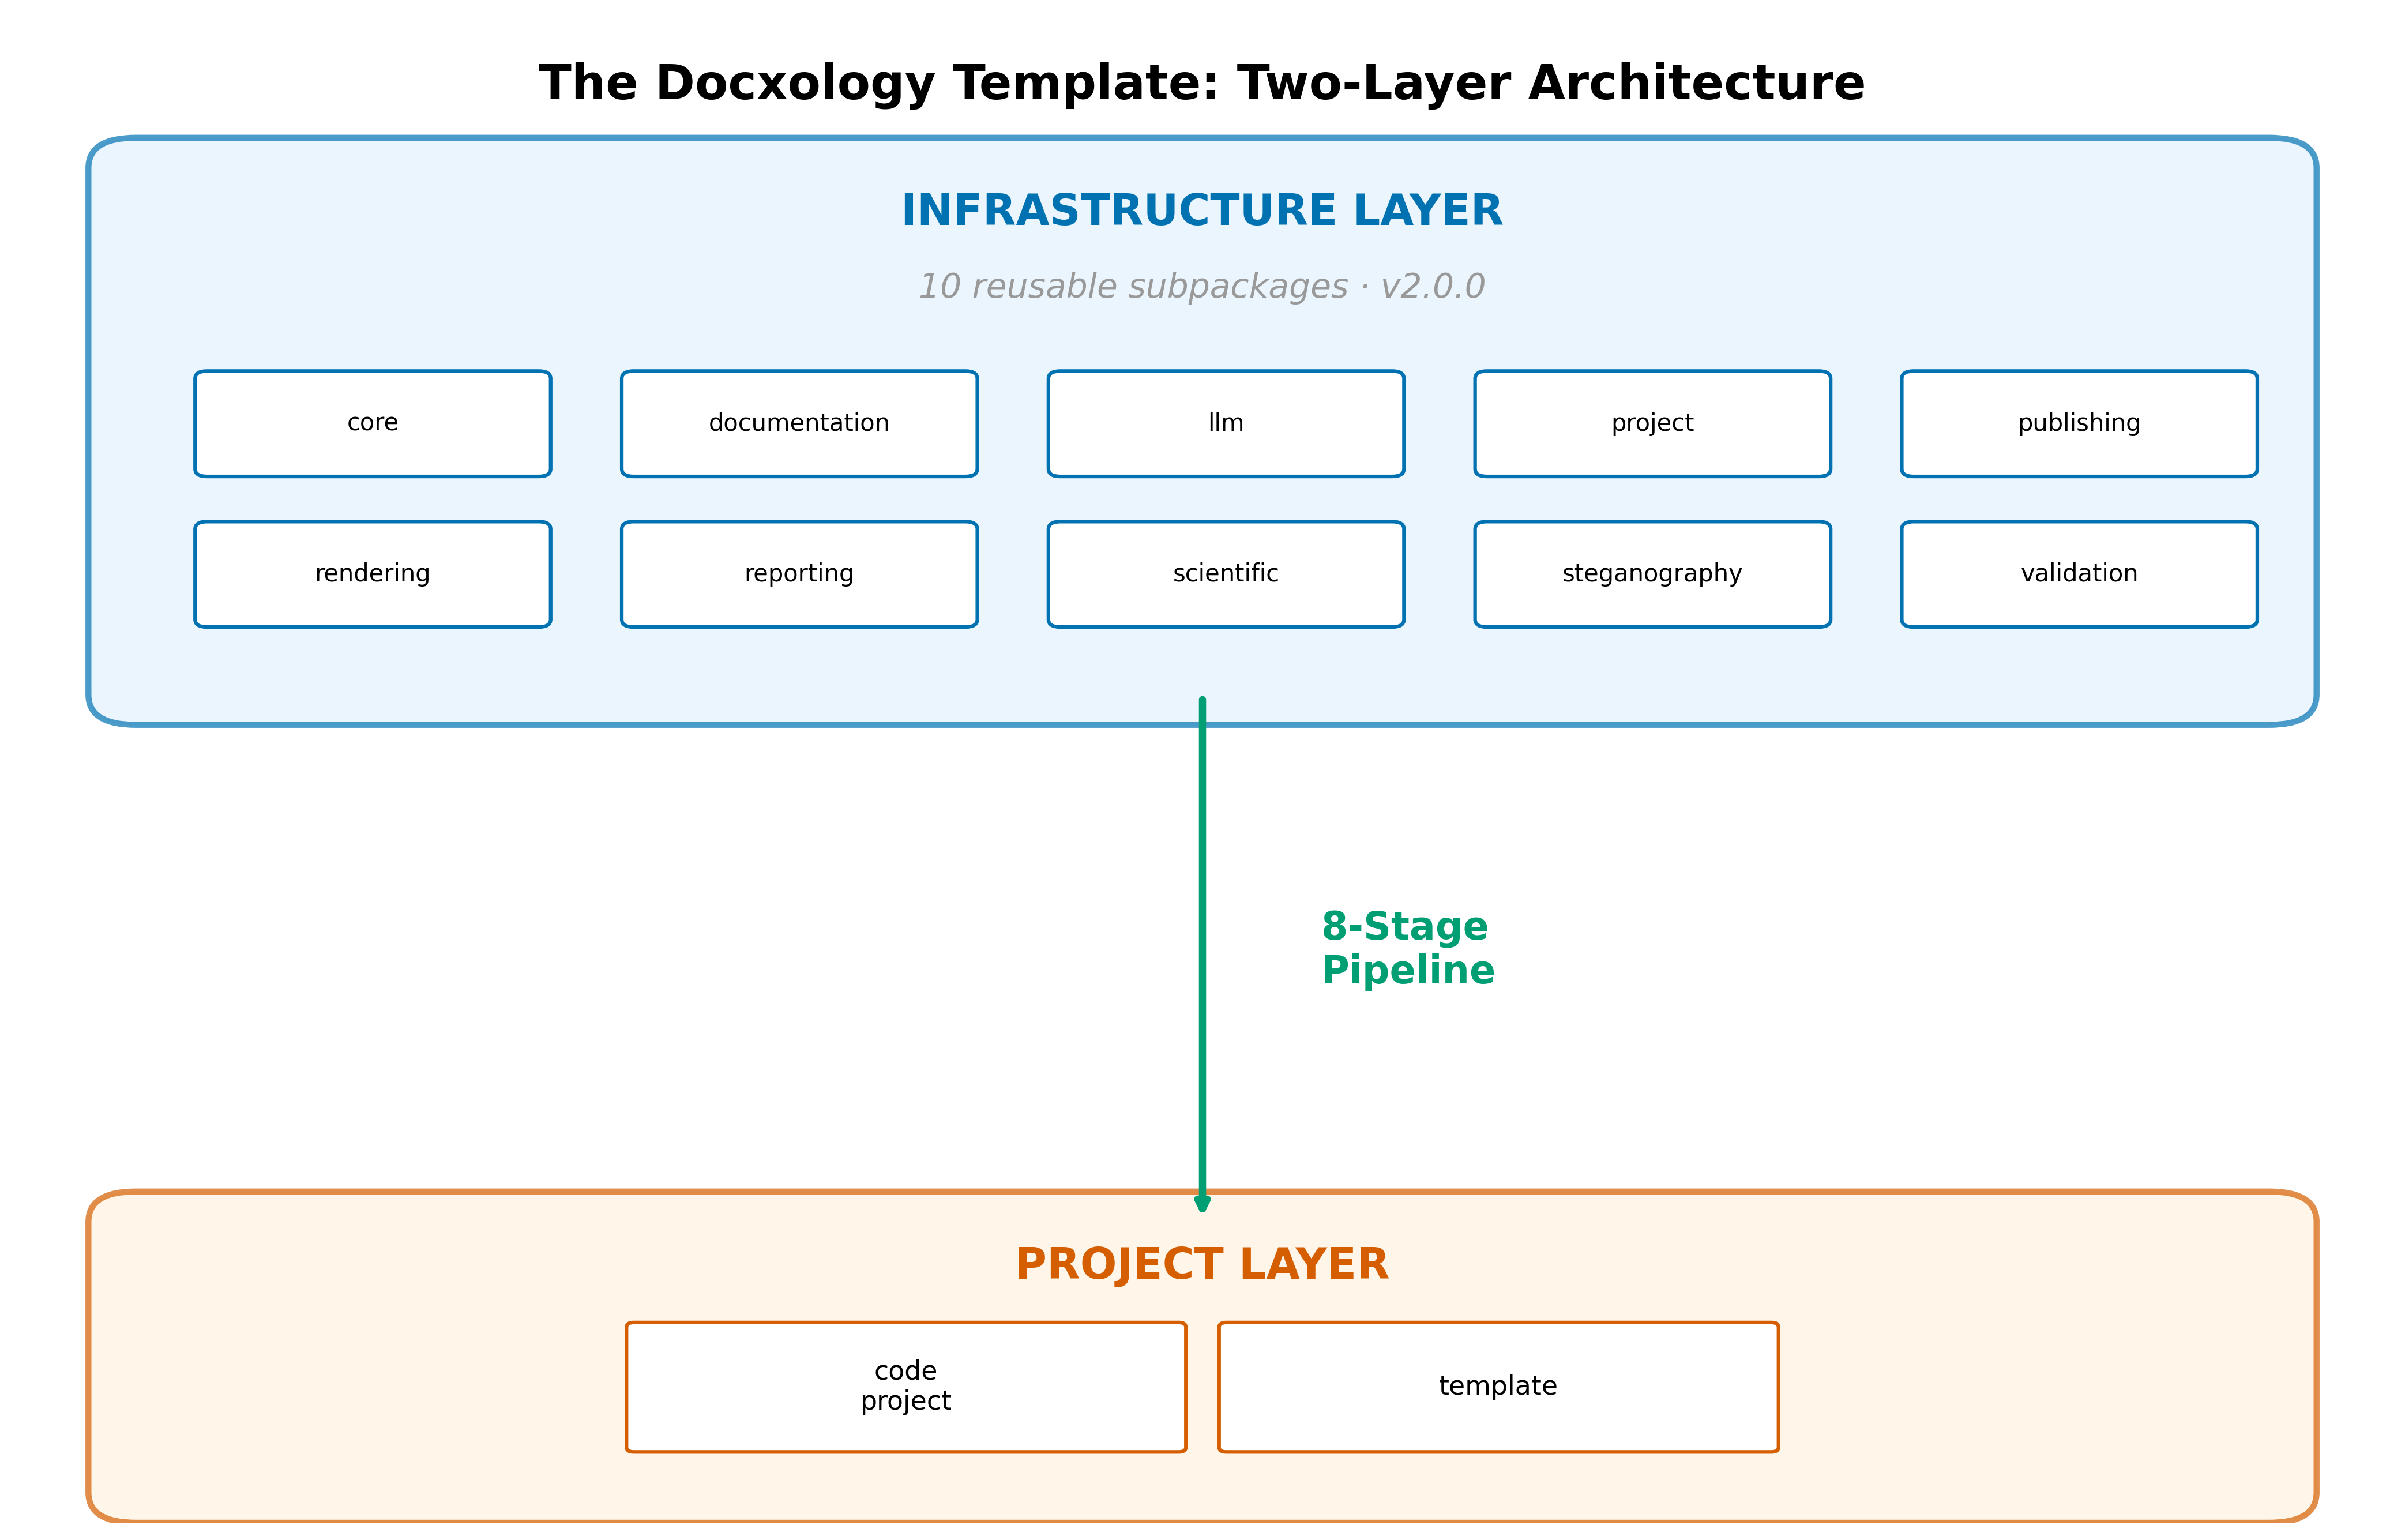
\includegraphics[keepaspectratio,alt={Two-Layer Architecture Overview}]{../figures/architecture_overview.png}}
\emph{Figure 1: The Two-Layer Architecture separating infrastructure
modules from project workspaces.}

\pandocbounded{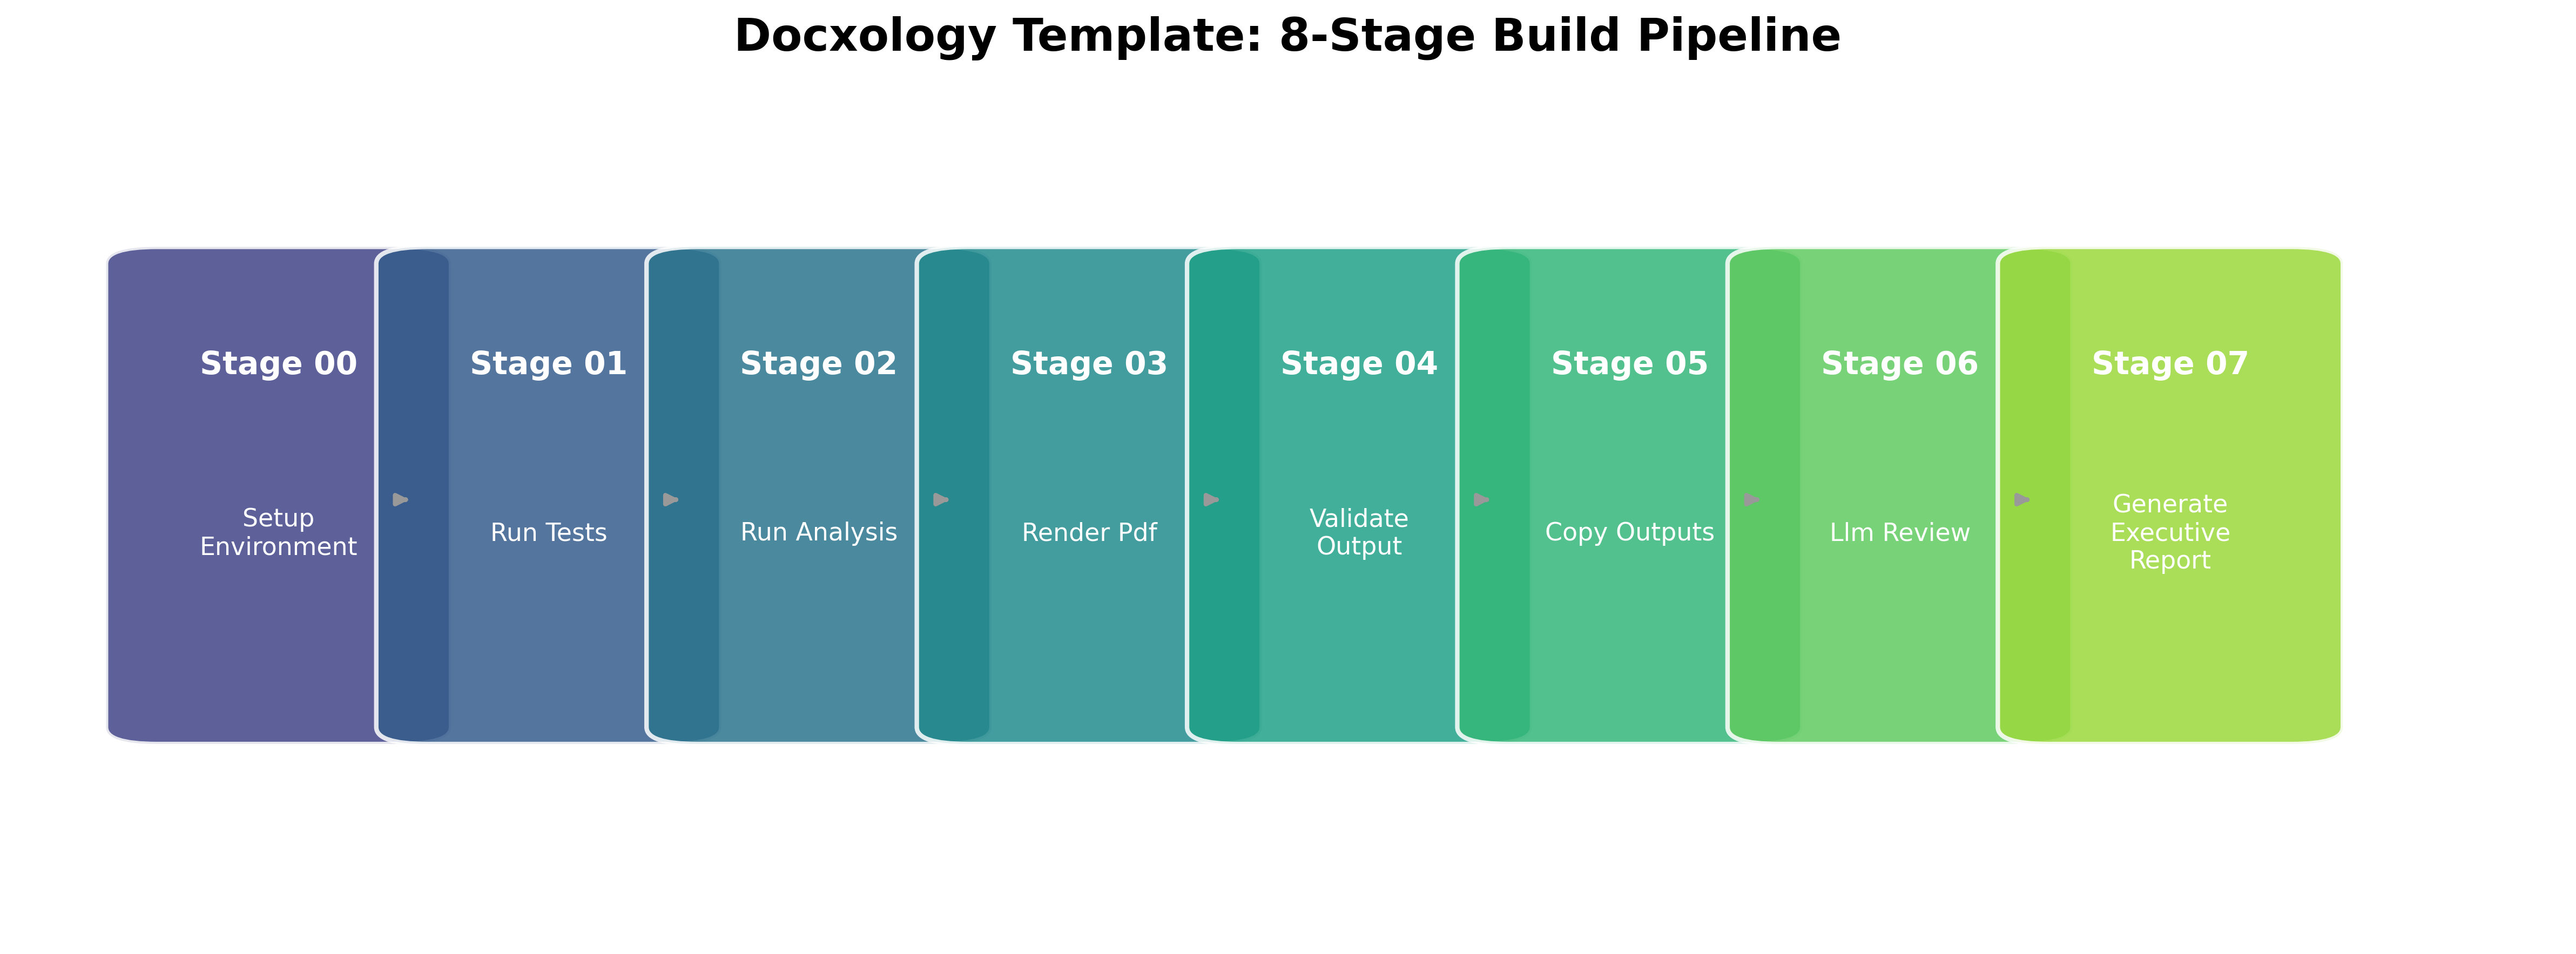
\includegraphics[keepaspectratio,alt={Pipeline Stage Flow}]{../figures/pipeline_stages.png}}
\emph{Figure 2: The eight-stage build pipeline from environment setup
through executive reporting.}

\pandocbounded{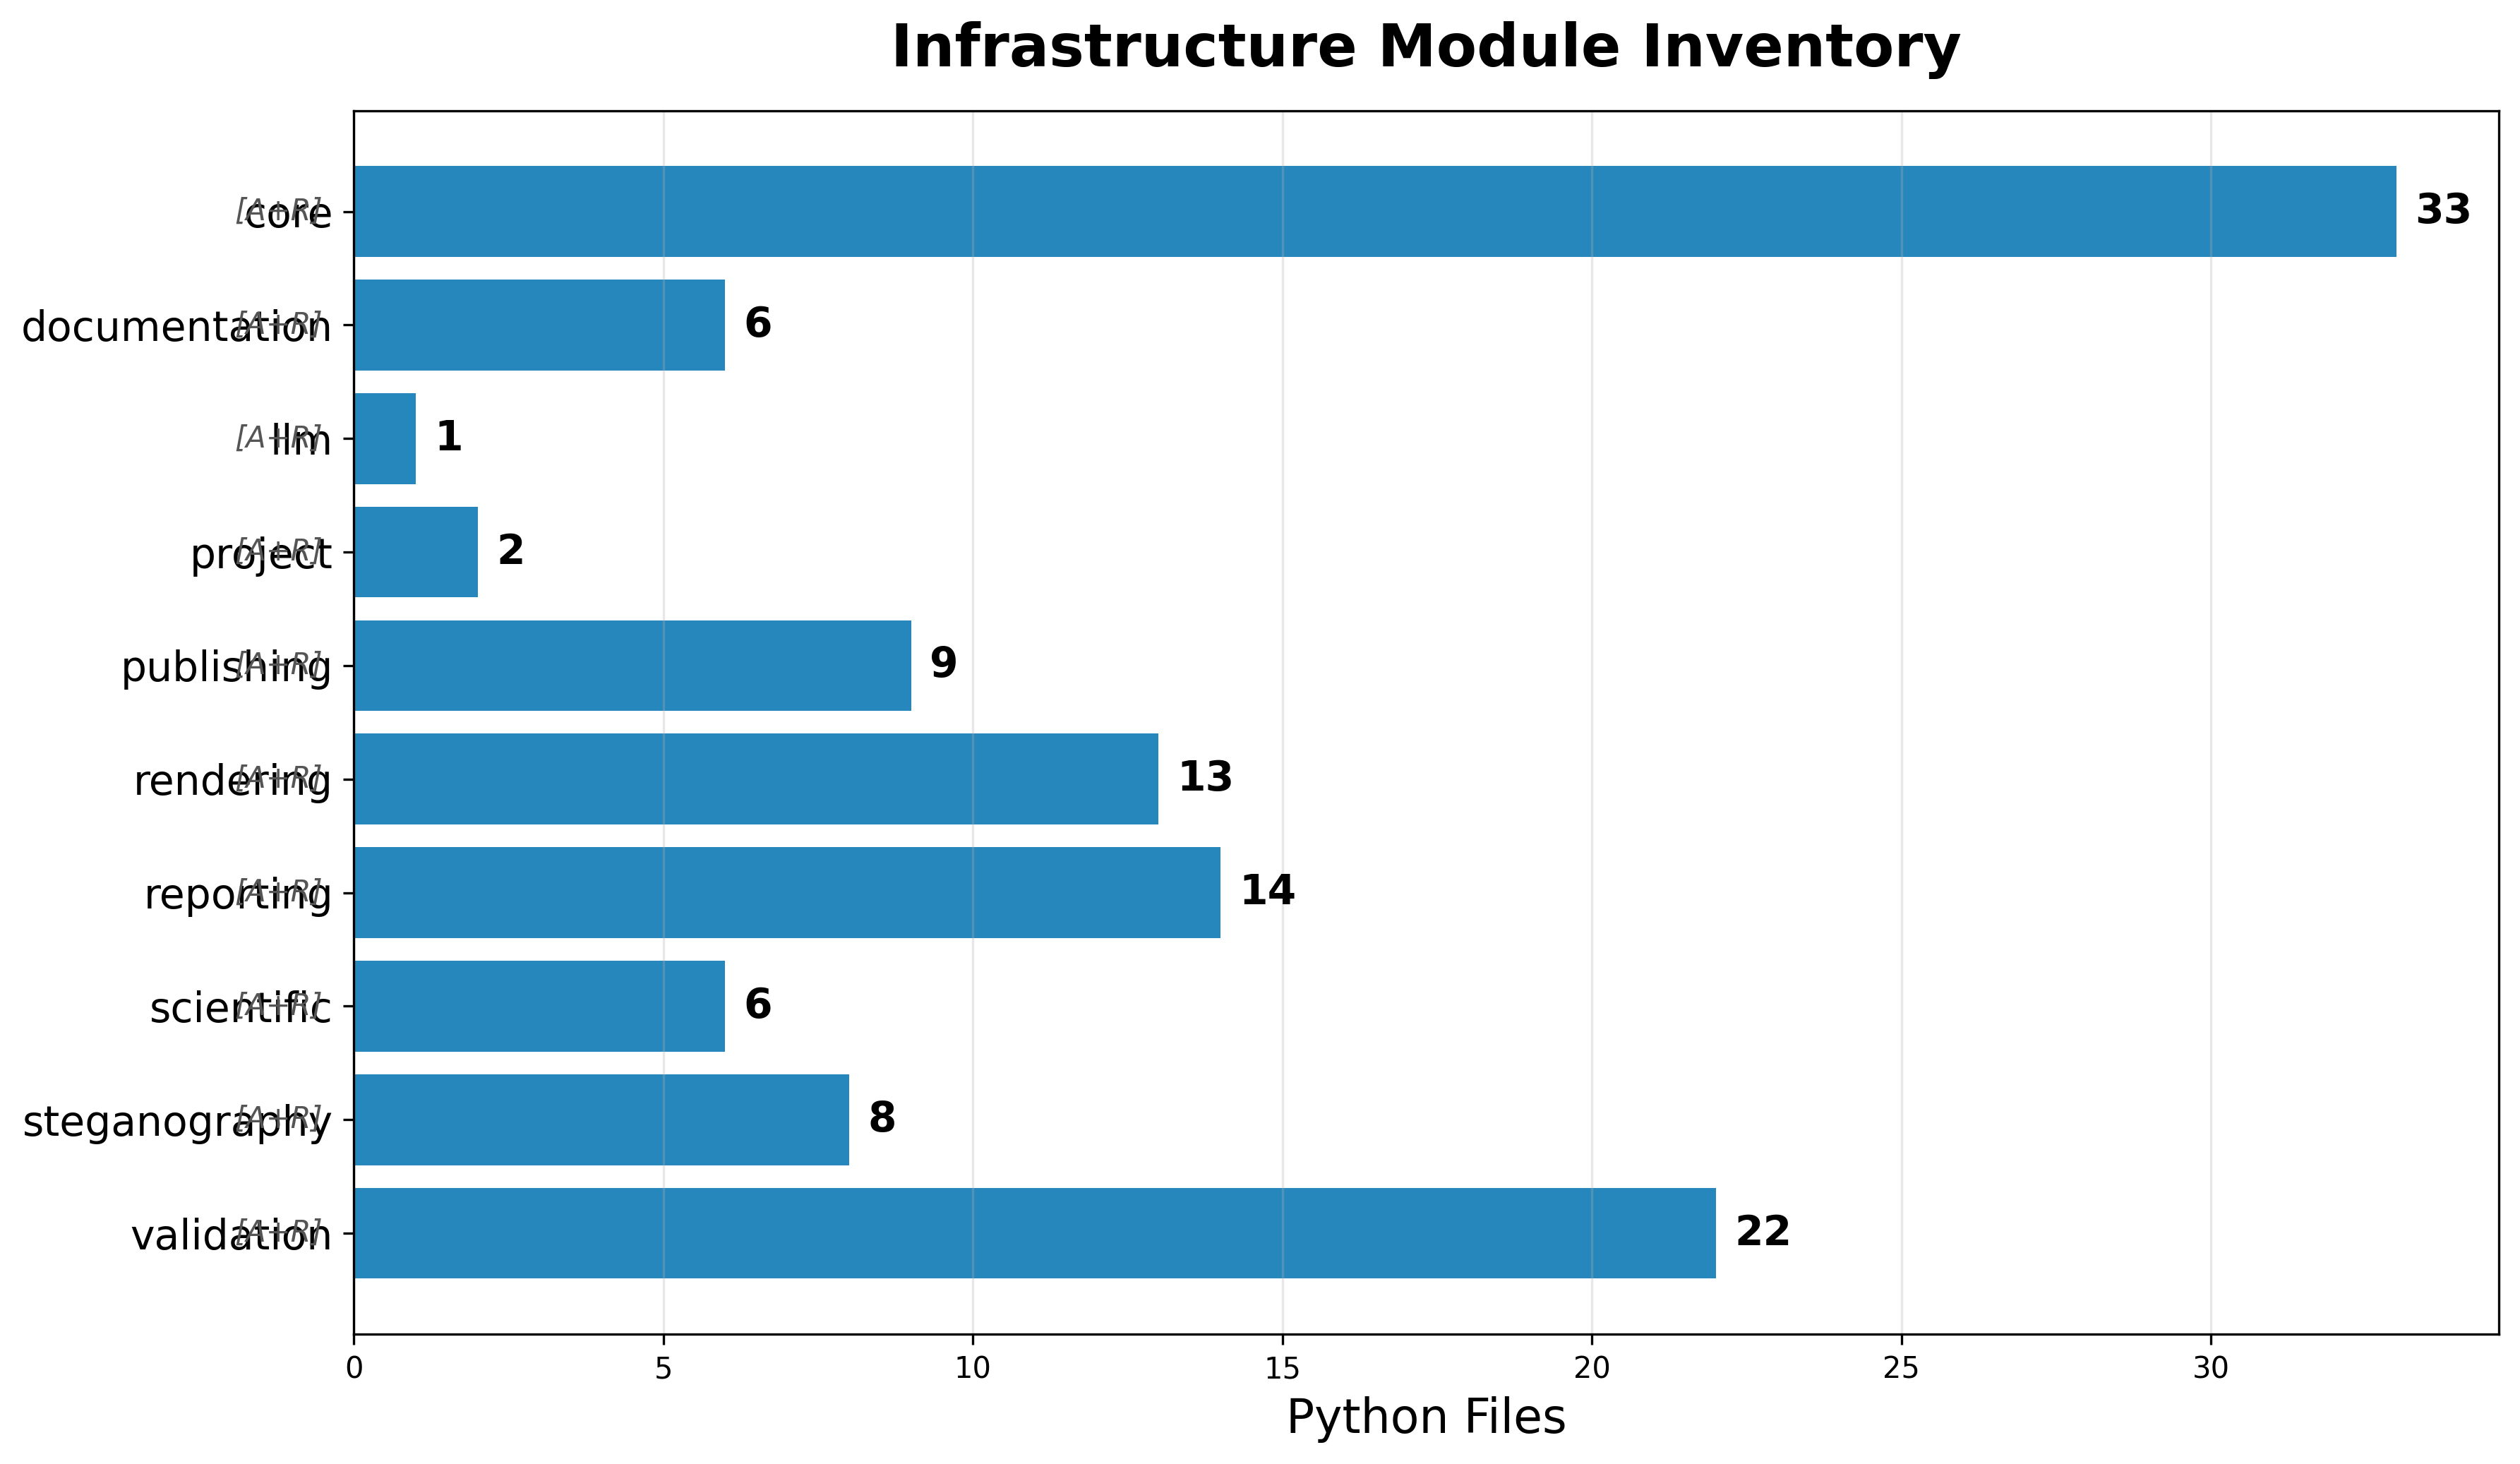
\includegraphics[keepaspectratio,alt={Infrastructure Module Inventory}]{../figures/module_inventory.png}}
\emph{Figure 3: Python file count per infrastructure module, with
documentation status indicators.}

\subsection{Comparative Feature
Analysis}\label{comparative-feature-analysis}

To contextualize the Docxology Template's contributions, we compare its
feature set against established tools:

{\def\LTcaptype{none} % do not increment counter
\begin{longtable}[]{@{}
  >{\raggedright\arraybackslash}p{(\linewidth - 12\tabcolsep) * \real{0.1324}}
  >{\centering\arraybackslash}p{(\linewidth - 12\tabcolsep) * \real{0.1618}}
  >{\centering\arraybackslash}p{(\linewidth - 12\tabcolsep) * \real{0.1618}}
  >{\centering\arraybackslash}p{(\linewidth - 12\tabcolsep) * \real{0.1471}}
  >{\centering\arraybackslash}p{(\linewidth - 12\tabcolsep) * \real{0.0735}}
  >{\centering\arraybackslash}p{(\linewidth - 12\tabcolsep) * \real{0.1176}}
  >{\centering\arraybackslash}p{(\linewidth - 12\tabcolsep) * \real{0.2059}}@{}}
\toprule\noalign{}
\begin{minipage}[b]{\linewidth}\raggedright
Feature
\end{minipage} & \begin{minipage}[b]{\linewidth}\centering
Docxology
\end{minipage} & \begin{minipage}[b]{\linewidth}\centering
Snakemake
\end{minipage} & \begin{minipage}[b]{\linewidth}\centering
Nextflow
\end{minipage} & \begin{minipage}[b]{\linewidth}\centering
CWL
\end{minipage} & \begin{minipage}[b]{\linewidth}\centering
Quarto
\end{minipage} & \begin{minipage}[b]{\linewidth}\centering
Jupyter Book
\end{minipage} \\
\midrule\noalign{}
\endhead
\bottomrule\noalign{}
\endlastfoot
Pipeline orchestration & ✓ & ✓ & ✓ & ✓ & --- & --- \\
Manuscript rendering & ✓ & --- & --- & --- & ✓ & ✓ \\
Testing enforcement & ✓ & --- & --- & --- & --- & --- \\
Coverage thresholds & ✓ & --- & --- & --- & --- & --- \\
Cryptographic provenance & ✓ & --- & --- & --- & --- & --- \\
Multi-project management & ✓ & --- & --- & --- & --- & --- \\
AI-agent documentation & ✓ & --- & --- & --- & --- & --- \\
Interactive TUI & ✓ & --- & --- & --- & --- & --- \\
Zero-mock policy & ✓ & --- & --- & --- & --- & --- \\
\end{longtable}
}

The Docxology Template is, to our knowledge, the only open-source system
that integrates all nine capabilities within a single cohesive
architecture.

\subsection{Test Quality Metrics}\label{test-quality-metrics}

The Zero-Mock testing policy produces measurably higher-fidelity tests:

\begin{itemize}
\tightlist
\item
  \textbf{Zero mock objects} across all test suites (verified by
  automated scanning for \texttt{unittest.mock}, \texttt{MagicMock}, and
  \texttt{patch} imports).
\item
  \textbf{Real filesystem operations}: Tests create, read, validate, and
  delete actual files in temporary directories.
\item
  \textbf{Real subprocess calls}: Pipeline stage tests invoke actual
  \texttt{pytest}, \texttt{pandoc}, and \texttt{xelatex} subprocesses.
\item
  \textbf{Marker-based skip logic}: Tests requiring optional services
  (Ollama, network) use \texttt{@pytest.mark.requires\_ollama} for
  graceful degradation.
\item
  \textbf{Categorical axiom verification}: The
  \texttt{cognitive\_case\_diagrams} project tests validate identity
  morphisms, composition, weight multiplication, and the triangle
  inequality on real enriched category objects.
\end{itemize}

\newpage

\section{Discussion}\label{discussion}

\subsection{The Zero-Mock Tradeoff}\label{the-zero-mock-tradeoff}

The Zero-Mock testing policy is the template's most distinctive design
decision. By prohibiting all mock objects, we gain confidence that tests
exercise real code paths---a pytest run against the template genuinely
invokes \texttt{pandoc}, writes to disk, and parses real YAML. The cost
is test duration: the full infrastructure test suite (3,053 tests) takes
2--4 minutes, compared to sub-second execution typical of heavily-mocked
suites.

We argue this tradeoff is strongly favorable for research software.
Unlike web applications where millisecond latency and thousands of daily
deploys demand fast feedback loops, research pipelines run infrequently
(once per manuscript revision) and correctness vastly outweighs speed. A
mocked test that passes while the real renderer fails is worse than a
slow test that catches the failure. As Peng \citep{peng2011reproducible}
argues, the standard for computational reproducibility is that results
can be independently verified---mock objects, by definition, prevent
such verification. Garijo et al.'s FAIRsoft evaluator
\citep{garijo2024fairsoft} identifies \emph{executability}---the ability
to actually install and run research software---as a primary quality
indicator, yet the majority of evaluated tools fail this test. The
Zero-Mock policy goes further: it requires not merely that the software
can be installed, but that every integration pathway has been exercised
against real dependencies under test.

However, the policy requires careful management of external
dependencies. Tests requiring Ollama (the local LLM backend) use
\texttt{@pytest.mark.requires\_ollama} and are skipped in environments
where the service is unavailable. This marker system preserves the
Zero-Mock principle while acknowledging that not all environments
provide all services.

\subsection{Scalability: From 1 to N
Projects}\label{scalability-from-1-to-n-projects}

The Standalone Project Paradigm enables horizontal scaling: adding a new
project requires creating a directory with
\texttt{manuscript/config.yaml} and nothing else. No infrastructure code
changes, no \texttt{pyproject.toml} modifications, no CI configuration
updates. The \texttt{run.sh} orchestrator automatically discovers new
projects and presents them in its interactive menu.

We have validated this scaling model with three heterogeneous projects:

\begin{itemize}
\tightlist
\item
  \textbf{\texttt{code\_project}}: Numerical optimization with gradient
  descent, 58 tests, 96.6\% coverage.
\item
  \textbf{\texttt{cognitive\_case\_diagrams}}: Category-theoretic
  linguistics with 25+ DisCoPy-generated figures from 17 renderers, 257
  tests, \textasciitilde96\% coverage, 79 BibTeX references spanning 17
  research areas.
\item
  \textbf{\texttt{template}}: This self-referential architectural
  analysis, 36 tests, 90\%+ coverage.
\end{itemize}

These projects share no code with each other. They share only the
infrastructure layer---ten modules, 137 Python files---which provides
logging, rendering, validation, steganography, and reporting services
identically to each project. This validates the Two-Layer Architecture's
claim that infrastructure and project concerns can be cleanly separated.

\subsection{Comparison to Existing
Tools}\label{comparison-to-existing-tools}

The Docxology Template occupies a unique niche in the reproducible
research ecosystem. Unlike Snakemake \citep{koster2012snakemake} and
Nextflow \citep{ditommaso2017nextflow}, which excel at parallelizing
computational pipelines but do not manage manuscript production or
testing enforcement, the template integrates the entire research
lifecycle from code to publication. Snakemake 8.x (2024) introduced a
plugin architecture for extended execution backends, yet its scope
remains computational workflow orchestration---it does not integrate
manuscript rendering, documentation standards, or cryptographic
provenance. Unlike Quarto \citep{allaire2024quarto} and R Markdown
\citep{xie2015dynamic}, which integrate code execution with document
rendering but do not enforce coverage thresholds or embed cryptographic
provenance, the template treats testing and provenance as first-class
architectural concerns rather than optional plugins.

The key differentiator is the \emph{enforcement} mechanism. The FAIR4RS
principles \citep{barker2022fair4rs} represent a significant advance in
articulating what research software quality requires---executability,
interoperability, comprehensive metadata---and FAIRsoft
\citep{garijo2024fairsoft} provides automated scoring against these
criteria. Yet FAIR4RS compliance is assessed observationally rather than
enforced architecturally: a tool may score well on FAIRsoft metrics
today and regress tomorrow without detection. The Docxology Template
operationalizes FAIR4RS by coupling quality metrics to pipeline gates:
the pipeline will not advance past Stage 01 if project test coverage
falls below 90\%. Provenance is not documented in a README; it is
cryptographically embedded in the PDF per the W3C PROV model's principle
that provenance should be machine-readable and tamper-evident
\citep{moreau2013provdm}. Documentation is not a best-effort companion;
it is a structural requirement enforced by the Documentation Duality
standard. In this sense, the template bridges the gap between FAIR4RS as
a descriptive standard and FAIR4RS as an enforced invariant.

In Gentleman and Temple Lang's terminology
\citep{gentleman2007research}, the Docxology Template is a
\emph{research compendium} scaled to the repository level---bundling not
just one study's code and data but N studies, with shared
infrastructure, automated testing, and embedded provenance. Nüst et
al.'s executable research compendium (ERC)
\citep{nust2017containerization} extends this vision with containerized
reproduction environments; the Docxology Template complements
containerization by adding the testing enforcement, multi-project
management, and provenance embedding layers that ERCs do not address.

\subsection{The AI Collaboration
Model}\label{the-ai-collaboration-model}

The Documentation Duality standard (\texttt{README.md} +
\texttt{AGENTS.md} at every directory level) emerged from practical
experience with AI coding assistants. Language models perform
significantly better when provided with structured, machine-readable
context about architectural constraints, API surfaces, and testing
requirements. The \texttt{AGENTS.md} files serve as a form of ``prompt
engineering embedded in the codebase''---they preempt common failure
modes such as hallucinated API signatures, violation of the Thin
Orchestrator pattern, and introduction of mock objects. Lau and Guo
\citep{lau2025aicoding} identify contextual code understanding as a
primary bottleneck across 90 surveyed AI coding assistant systems; the
Documentation Duality standard addresses this by providing
pre-structured context at every directory level, reducing the surface
area for hallucination.

This model creates a positive feedback loop: as AI agents modify the
codebase, they update the corresponding documentation, which in turn
provides better context for future modifications. The supplementary
\texttt{CLAUDE.md} file at the repository root provides system-level
instructions (the Two-Layer Architecture, Zero-Mock policy, naming
conventions) that apply globally, creating a three-tier documentation
architecture:

\begin{enumerate}
\def\labelenumi{\arabic{enumi}.}
\tightlist
\item
  \textbf{Repository-level} (\texttt{CLAUDE.md}): Global constraints and
  architectural principles.
\item
  \textbf{Directory-level} (\texttt{AGENTS.md}): Local API surfaces,
  file inventories, and integration patterns.
\item
  \textbf{Human-level} (\texttt{README.md}): Quick-start guides and
  navigation aids.
\end{enumerate}

This three-tier model is, to our knowledge, novel in the research
software engineering literature. As AI coding assistants evolve from
reactive suggestion engines toward agentic systems capable of autonomous
multi-file modifications \citep{lau2025aicoding}, the need for
machine-readable architectural context becomes not a convenience but a
prerequisite for safe AI-assisted software evolution.

\subsection{The Learning Curve}\label{the-learning-curve}

The Thin Orchestrator pattern imposes a cognitive overhead on
researchers accustomed to writing monolithic scripts. The requirement to
factor all logic into \texttt{src/} modules and use scripts only as
stateless wiring introduces an additional layer of indirection. We
mitigate this through:

\begin{enumerate}
\def\labelenumi{\arabic{enumi}.}
\tightlist
\item
  \textbf{Template examples}: The \texttt{code\_project} serves as a
  fully worked exemplar with comprehensive comments.
\item
  \textbf{Documentation Duality}: Every directory has both
  \texttt{README.md} (for humans) and \texttt{AGENTS.md} (for AI
  collaborators), reducing the cost of navigation.
\item
  \textbf{Interactive orchestrator}: \texttt{run.sh} provides a TUI menu
  that abstracts pipeline complexity.
\item
  \textbf{Skill-level documentation}: The \texttt{docs/guides/}
  directory provides four progressive guides (Levels 1--3 Beginner, 4--6
  Intermediate, 7--9 Advanced, 10--12 Expert) alongside a comprehensive
  new-project setup checklist.
\end{enumerate}

\subsection{Limitations}\label{limitations}

\begin{itemize}
\tightlist
\item
  \textbf{LaTeX dependency}: The rendering pipeline requires a full TeX
  distribution (TeX Live or MiKTeX), which is a 4--6 GB install. This is
  the largest single dependency.
\item
  \textbf{Python-centric}: The infrastructure layer is Python-only.
  Projects in other languages can use the rendering and steganography
  stages but cannot leverage the \texttt{scientific} or
  \texttt{validation} modules.
\item
  \textbf{Single-machine}: The pipeline runs locally. Distributed
  execution (e.g., across a compute cluster) is not natively supported.
\item
  \textbf{Steganographic robustness}: Alpha-channel overlays are
  stripped by aggressive PDF optimization tools (e.g.,
  \texttt{qpdf\ -\/-optimize}). QR codes are visible and removable.
  Neither provides non-repudiation without digital signatures.
\item
  \textbf{Test duration}: The Zero-Mock policy increases test execution
  time from sub-second (mocked) to multi-minute (real) for the full
  infrastructure suite. This is acceptable for research workflows but
  may not suit continuous deployment scenarios.
\end{itemize}

\subsection{Future Directions}\label{future-directions}

\begin{enumerate}
\def\labelenumi{\arabic{enumi}.}
\tightlist
\item
  \textbf{Supply-chain provenance}: Integration with software supply
  chain frameworks such as in-toto \citep{torresarias2019intoto} and
  SLSA (Supply-chain Levels for Software Artifacts) to provide
  end-to-end attestation from source commit through build pipeline to
  published artifact. The template's existing steganographic layer
  embeds document-level provenance; supply-chain frameworks would add
  build-level provenance, closing the gap between ``this PDF was
  produced by this pipeline'' and ``this pipeline was executed with this
  verified source code.''
\item
  \textbf{Decentralized provenance}: Integration with IPFS or Arweave
  for immutable publication records, extending the SHA-256-based tamper
  detection to content-addressed storage networks.
\item
  \textbf{Digital signatures}: GPG or X.509 signing integrated into the
  steganographic layer, providing cryptographic non-repudiation in
  addition to tamper detection.
\item
  \textbf{Continuous integration}: GitHub Actions workflows that execute
  the pipeline on every push, with PDF artifacts as release assets and
  automated DOI registration via Zenodo.
\item
  \textbf{Multi-language support}: Extension of the Thin Orchestrator
  pattern to R, Julia, and Rust projects, enabling polyglot research
  workflows within the Two-Layer Architecture.
\item
  \textbf{Automated FAIR4RS assessment}: Periodic self-scoring against
  FAIRsoft metrics \citep{garijo2024fairsoft}, with quality indicators
  (executability, documentation completeness, metadata richness) tracked
  as pipeline artifacts alongside test coverage and rendering status.
\item
  \textbf{Knowledge graph integration}: Connecting pipeline outputs to
  Active Inference Knowledge Base entries for automated meta-analysis
  and cross-project citation tracking.
\item
  \textbf{Formal verification}: Static analysis tooling to enforce the
  Thin Orchestrator pattern---verifying that scripts contain no
  algorithmic logic and that \texttt{src/} modules do not import from
  \texttt{scripts/}.
\end{enumerate}

\section{Conclusion}\label{conclusion}

The Docxology Template demonstrates that high-integrity, reproducible
research need not be onerous. By embedding provenance, testing, and
documentation into the architecture itself---rather than layering them
atop a fragmented workflow---the template transforms ``best practices''
from aspirational guidelines into enforced invariants
\citep{wilson2017good, sandve2013ten}. The Two-Layer Architecture
ensures that infrastructure improvements propagate to all projects
without coupling. The Zero-Mock policy ensures that tests reflect
reality. The steganographic provenance layer ensures that published
artifacts carry their own authentication. The FAIR4RS principles
\citep{barker2022fair4rs} articulate what research software quality
requires; the Docxology Template demonstrates how to enforce it.

The template is not merely a build tool; it is an epistemological
commitment. It asserts that a research paper is not a static document
but a build artifact---reproducible, verifiable, and traceable to the
code that generated it. As Knuth observed, programs should be written
for humans to read and only incidentally for machines to execute
\citep{knuth1984literate}. We extend this dictum: research manuscripts
should be \emph{built} for verification and only incidentally for
reading. In an era of generative AI and synthetic media, where the
boundary between human-authored and machine-generated text grows
increasingly indeterminate \citep{gruenpeter2021research}, the
provenance chain from source code to published PDF is not an
administrative convenience---it is the epistemic ground on which
scientific trust must be rebuilt.

\newpage

\section{Infrastructure Module
Reference}\label{infrastructure-module-reference}

This section provides a detailed reference for all ten infrastructure
subpackages, documenting their purpose, key classes, public API, and
integration points within the pipeline. The infrastructure layer
comprises 137 Python modules validated by 3,053 tests.

\subsection{\texorpdfstring{\texttt{infrastructure.core} (28
modules)}{infrastructure.core (28 modules)}}\label{infrastructure.core-28-modules}

\textbf{Purpose}: Foundation utilities providing the bedrock services
consumed by all other modules and all projects.

\textbf{Key Components}:

{\def\LTcaptype{none} % do not increment counter
\begin{longtable}[]{@{}
  >{\raggedright\arraybackslash}p{(\linewidth - 2\tabcolsep) * \real{0.5500}}
  >{\raggedright\arraybackslash}p{(\linewidth - 2\tabcolsep) * \real{0.4500}}@{}}
\toprule\noalign{}
\begin{minipage}[b]{\linewidth}\raggedright
Component
\end{minipage} & \begin{minipage}[b]{\linewidth}\raggedright
Purpose
\end{minipage} \\
\midrule\noalign{}
\endhead
\bottomrule\noalign{}
\endlastfoot
\texttt{logging\_utils.py} & Structured logger factory
(\texttt{get\_logger}) with colored console output and file rotation \\
\texttt{config\_loader.py} & YAML config parser (\texttt{load\_config})
with schema validation and default merging \\
\texttt{exceptions.py} & Exception hierarchy: \texttt{TemplateError} →
\texttt{ConfigurationError}, \texttt{ValidationError},
\texttt{BuildError} \\
\texttt{environment.py} & Environment detection, Python command
resolution, \texttt{PYTHONPATH} management \\
\texttt{progress.py} & \texttt{ProgressBar} for pipeline stage progress
reporting \\
\texttt{checkpoint.py} & \texttt{CheckpointManager} for resumable
pipeline execution \\
\texttt{health.py} & \texttt{SystemHealthChecker} for pre-pipeline
dependency validation \\
\texttt{performance.py} & \texttt{monitor\_performance} context manager
for timing and memory tracking \\
\texttt{\_optional\_deps.py} & Lazy loading of optional dependencies
(\texttt{psutil}, \texttt{reportlab}) \\
\end{longtable}
}

\textbf{Integration}: Every module and script imports from
\texttt{core}. The exception hierarchy is used for pipeline flow
control---\texttt{ValidationError} triggers stage failure,
\texttt{BuildError} halts the entire pipeline. The lazy loader in
\texttt{\_optional\_deps.py} separates core imports from optional
subpackages, preventing cascading import failures in environments with
partial dependency sets.

\subsection{\texorpdfstring{\texttt{infrastructure.documentation} (6
modules)}{infrastructure.documentation (6 modules)}}\label{infrastructure.documentation-6-modules}

\textbf{Purpose}: Documentation management, figure registration, and API
glossary generation.

\textbf{Key Components}:

{\def\LTcaptype{none} % do not increment counter
\begin{longtable}[]{@{}
  >{\raggedright\arraybackslash}p{(\linewidth - 2\tabcolsep) * \real{0.5500}}
  >{\raggedright\arraybackslash}p{(\linewidth - 2\tabcolsep) * \real{0.4500}}@{}}
\toprule\noalign{}
\begin{minipage}[b]{\linewidth}\raggedright
Component
\end{minipage} & \begin{minipage}[b]{\linewidth}\raggedright
Purpose
\end{minipage} \\
\midrule\noalign{}
\endhead
\bottomrule\noalign{}
\endlastfoot
\texttt{figure\_manager.py} & \texttt{FigureManager} --- maintains a
JSON registry of all generated figures with captions, labels, and
generation metadata \\
\texttt{glossary\_gen.py} & \texttt{generate\_glossary} --- programmatic
API glossary extraction from Python source files \\
\end{longtable}
}

\textbf{Integration}: Called by project scripts during Stage 02 to
register figures for automated cross-referencing in the manuscript. The
glossary generator supports the Documentation Duality standard by
extracting docstrings and function signatures.

\subsection{\texorpdfstring{\texttt{infrastructure.llm} (30
modules)}{infrastructure.llm (30 modules)}}\label{infrastructure.llm-30-modules}

\textbf{Purpose}: Local LLM integration for automated manuscript review,
translation, and literature search.

\textbf{Key Components}:

{\def\LTcaptype{none} % do not increment counter
\begin{longtable}[]{@{}
  >{\raggedright\arraybackslash}p{(\linewidth - 2\tabcolsep) * \real{0.5500}}
  >{\raggedright\arraybackslash}p{(\linewidth - 2\tabcolsep) * \real{0.4500}}@{}}
\toprule\noalign{}
\begin{minipage}[b]{\linewidth}\raggedright
Component
\end{minipage} & \begin{minipage}[b]{\linewidth}\raggedright
Purpose
\end{minipage} \\
\midrule\noalign{}
\endhead
\bottomrule\noalign{}
\endlastfoot
\texttt{review.py} & Executive summary and quality review generation \\
\texttt{translation.py} & Abstract translation into configured target
languages \\
\texttt{client.py} & Ollama HTTP client with retry logic and timeout
management \\
\texttt{literature/} & Literature search subpackage with semantic query
support \\
\texttt{templates/} & Prompt templates for structured LLM
interactions \\
\end{longtable}
}

\textbf{Integration}: Invoked during Stage 06. Requires a running Ollama
instance. Gracefully degrades when unavailable. The literature search
subpackage enables programmatic discovery of related work during
manuscript preparation.

\subsection{\texorpdfstring{\texttt{infrastructure.project} (2
modules)}{infrastructure.project (2 modules)}}\label{infrastructure.project-2-modules}

\textbf{Purpose}: Project discovery and workspace management.

\textbf{Key Components}:

{\def\LTcaptype{none} % do not increment counter
\begin{longtable}[]{@{}
  >{\raggedright\arraybackslash}p{(\linewidth - 2\tabcolsep) * \real{0.5500}}
  >{\raggedright\arraybackslash}p{(\linewidth - 2\tabcolsep) * \real{0.4500}}@{}}
\toprule\noalign{}
\begin{minipage}[b]{\linewidth}\raggedright
Component
\end{minipage} & \begin{minipage}[b]{\linewidth}\raggedright
Purpose
\end{minipage} \\
\midrule\noalign{}
\endhead
\bottomrule\noalign{}
\endlastfoot
\texttt{discovery.py} & \texttt{\_discover\_project} --- finds valid
project directories by scanning for \texttt{manuscript/config.yaml} \\
\texttt{workspace.py} & Workspace initialization and cleanup
utilities \\
\end{longtable}
}

\textbf{Integration}: Used by \texttt{execute\_pipeline.py} and
\texttt{run.sh} to identify which projects can be built. The discovery
algorithm enforces the Standalone Project Paradigm: a directory is a
valid project if and only if it contains
\texttt{manuscript/config.yaml}.

\subsection{\texorpdfstring{\texttt{infrastructure.publishing} (9
modules)}{infrastructure.publishing (9 modules)}}\label{infrastructure.publishing-9-modules}

\textbf{Purpose}: Academic publishing metadata and citation generation.

\textbf{Key Components}:

{\def\LTcaptype{none} % do not increment counter
\begin{longtable}[]{@{}
  >{\raggedright\arraybackslash}p{(\linewidth - 2\tabcolsep) * \real{0.5500}}
  >{\raggedright\arraybackslash}p{(\linewidth - 2\tabcolsep) * \real{0.4500}}@{}}
\toprule\noalign{}
\begin{minipage}[b]{\linewidth}\raggedright
Component
\end{minipage} & \begin{minipage}[b]{\linewidth}\raggedright
Purpose
\end{minipage} \\
\midrule\noalign{}
\endhead
\bottomrule\noalign{}
\endlastfoot
\texttt{models.py} & \texttt{PublicationMetadata} dataclass with direct
attribute access and dynamic \texttt{getattr} fallback \\
\texttt{citations.py} & \texttt{generate\_citation\_apa},
\texttt{generate\_citation\_bibtex}, \texttt{generate\_citation\_mla} \\
\texttt{zenodo.py} & Zenodo API integration for DOI registration \\
\end{longtable}
}

\textbf{Integration}: Used during Stage 02 by analysis scripts to
extract publishable metadata from results. Citation generators produce
correctly formatted strings from \texttt{config.yaml} metadata.

\subsection{\texorpdfstring{\texttt{infrastructure.rendering} (12
modules)}{infrastructure.rendering (12 modules)}}\label{infrastructure.rendering-12-modules}

\textbf{Purpose}: Multi-format document rendering (Markdown → LaTeX →
PDF, HTML reports).

\textbf{Key Components}:

{\def\LTcaptype{none} % do not increment counter
\begin{longtable}[]{@{}
  >{\raggedright\arraybackslash}p{(\linewidth - 2\tabcolsep) * \real{0.5500}}
  >{\raggedright\arraybackslash}p{(\linewidth - 2\tabcolsep) * \real{0.4500}}@{}}
\toprule\noalign{}
\begin{minipage}[b]{\linewidth}\raggedright
Component
\end{minipage} & \begin{minipage}[b]{\linewidth}\raggedright
Purpose
\end{minipage} \\
\midrule\noalign{}
\endhead
\bottomrule\noalign{}
\endlastfoot
\texttt{pandoc.py} & Pandoc invocation with custom filters and metadata
injection \\
\texttt{latex.py} & XeLaTeX compilation with auxiliary file management
and stale \texttt{.aux} cleanup \\
\texttt{pdf\_builder.py} & End-to-end PDF construction orchestrating
Pandoc and XeLaTeX \\
\texttt{html\_report.py} & HTML executive report generation \\
\texttt{markdown\_report.py} & Markdown-format report generation \\
\end{longtable}
}

\textbf{Integration}: Core of Stage 03. Reads \texttt{manuscript/*.md}
and \texttt{config.yaml}, produces
\texttt{output/\textless{}project\textgreater{}.pdf}. The auxiliary file
cleanup resolves a known rendering hazard where stale \texttt{.aux}
files cause ``Division by 0'' LaTeX errors.

\subsection{\texorpdfstring{\texttt{infrastructure.reporting} (14
modules)}{infrastructure.reporting (14 modules)}}\label{infrastructure.reporting-14-modules}

\textbf{Purpose}: Pipeline reporting, test result aggregation, and
coverage analysis.

\textbf{Key Components}:

{\def\LTcaptype{none} % do not increment counter
\begin{longtable}[]{@{}
  >{\raggedright\arraybackslash}p{(\linewidth - 2\tabcolsep) * \real{0.5500}}
  >{\raggedright\arraybackslash}p{(\linewidth - 2\tabcolsep) * \real{0.4500}}@{}}
\toprule\noalign{}
\begin{minipage}[b]{\linewidth}\raggedright
Component
\end{minipage} & \begin{minipage}[b]{\linewidth}\raggedright
Purpose
\end{minipage} \\
\midrule\noalign{}
\endhead
\bottomrule\noalign{}
\endlastfoot
\texttt{coverage\_parser.py} & Cascading parse strategies for pytest
output: \texttt{\_parse\_failures\_section},
\texttt{\_parse\_failures\_verbose}, \texttt{\_parse\_failures\_short},
\texttt{\_parse\_failures\_timeout},
\texttt{\_parse\_failures\_fallback} \\
\texttt{report\_generator.py} & Executive report generation in JSON and
Markdown \\
\texttt{statistics.py} & \texttt{collect\_output\_statistics} ---
enumerates output directory contents \\
\end{longtable}
}

\textbf{Integration}: Used during Stages 01, 04, and 07 for test result
parsing, validation reporting, and executive summary generation. The
cascading parser handles all pytest output formats robustly, falling
through five strategies to ensure no test failure is silently missed.

\subsection{\texorpdfstring{\texttt{infrastructure.scientific} (6
modules)}{infrastructure.scientific (6 modules)}}\label{infrastructure.scientific-6-modules}

\textbf{Purpose}: Scientific computing utilities for numerical analysis
and benchmarking.

\textbf{Key Components}:

{\def\LTcaptype{none} % do not increment counter
\begin{longtable}[]{@{}
  >{\raggedright\arraybackslash}p{(\linewidth - 2\tabcolsep) * \real{0.5500}}
  >{\raggedright\arraybackslash}p{(\linewidth - 2\tabcolsep) * \real{0.4500}}@{}}
\toprule\noalign{}
\begin{minipage}[b]{\linewidth}\raggedright
Component
\end{minipage} & \begin{minipage}[b]{\linewidth}\raggedright
Purpose
\end{minipage} \\
\midrule\noalign{}
\endhead
\bottomrule\noalign{}
\endlastfoot
\texttt{stability.py} & \texttt{check\_numerical\_stability} --- tests
functions for NaN/Inf behavior across input ranges \\
\texttt{benchmarking.py} & \texttt{benchmark\_function} --- measures
execution time and memory usage \\
\texttt{simulation.py} & Scientific simulation framework with parameter
sweeps \\
\end{longtable}
}

\textbf{Integration}: Used by \texttt{code\_project}'s analysis scripts
during Stage 02 for algorithm validation. The stability checker is
critical for ensuring that numerical results are reproducible across
different floating-point environments.

\subsection{\texorpdfstring{\texttt{infrastructure.steganography} (8
modules)}{infrastructure.steganography (8 modules)}}\label{infrastructure.steganography-8-modules}

\textbf{Purpose}: Cryptographic watermarking and provenance embedding
for PDF artifacts.

\textbf{Key Components}:

{\def\LTcaptype{none} % do not increment counter
\begin{longtable}[]{@{}
  >{\raggedright\arraybackslash}p{(\linewidth - 2\tabcolsep) * \real{0.5500}}
  >{\raggedright\arraybackslash}p{(\linewidth - 2\tabcolsep) * \real{0.4500}}@{}}
\toprule\noalign{}
\begin{minipage}[b]{\linewidth}\raggedright
Component
\end{minipage} & \begin{minipage}[b]{\linewidth}\raggedright
Purpose
\end{minipage} \\
\midrule\noalign{}
\endhead
\bottomrule\noalign{}
\endlastfoot
\texttt{metadata.py} & \texttt{inject\_pdf\_metadata} --- embeds XMP
metadata and PDF Info dictionary entries \\
\texttt{config.py} & \texttt{DocumentMetadata} dataclass for
steganography configuration \\
\texttt{overlay.py} & Alpha-channel text overlay with build timestamp
and commit hash \\
\texttt{qr.py} & QR code generation and injection into PDF pages \\
\texttt{hash.py} & SHA-256/SHA-512 hash computation for tamper
detection \\
\end{longtable}
}

\textbf{Integration}: Invoked by \texttt{secure\_run.sh} after the main
pipeline completes. Reads the rendered PDF and produces a
steganographically watermarked copy with an accompanying
\texttt{.hashes.json} manifest.

\subsection{\texorpdfstring{\texttt{infrastructure.validation} (22
modules)}{infrastructure.validation (22 modules)}}\label{infrastructure.validation-22-modules}

\textbf{Purpose}: Quality assurance and integrity verification for all
pipeline artifacts.

\textbf{Key Components}:

{\def\LTcaptype{none} % do not increment counter
\begin{longtable}[]{@{}
  >{\raggedright\arraybackslash}p{(\linewidth - 2\tabcolsep) * \real{0.5500}}
  >{\raggedright\arraybackslash}p{(\linewidth - 2\tabcolsep) * \real{0.4500}}@{}}
\toprule\noalign{}
\begin{minipage}[b]{\linewidth}\raggedright
Component
\end{minipage} & \begin{minipage}[b]{\linewidth}\raggedright
Purpose
\end{minipage} \\
\midrule\noalign{}
\endhead
\bottomrule\noalign{}
\endlastfoot
\texttt{pdf\_validator.py} & PDF structural integrity checking (xref
table, trailer, page count) \\
\texttt{markdown\_validator.py} & Markdown linting (heading hierarchy,
link integrity, orphan references) \\
\texttt{integrity.py} & \texttt{verify\_output\_integrity} ---
comprehensive output directory validation \\
\texttt{cli.py} & Command-line interface for standalone validation
operations \\
\end{longtable}
}

\textbf{Integration}: Core of Stage 04. Validates all generated
artifacts before they are finalized. The validation module is the most
module-dense package (22 files), reflecting the breadth of integrity
checks required across PDF, Markdown, image, and manifest formats.

\newpage

\section{Security and Provenance}\label{security-and-provenance}

Research integrity requires more than reproducibility; it requires
verifiable authorship. In an era of generative AI, automated scraping,
and synthetic media, the ability to prove that a document was produced
by a specific pipeline at a specific time is a critical defense against
fabrication and misattribution. The W3C PROV data model
\citep{moreau2013provdm} establishes a formal vocabulary for expressing
provenance records---entities, activities, and agents connected by
derivation, generation, and attribution relations. The Docxology
Template implements a domain-specific provenance layer that embeds these
relations directly into the PDF artifact itself, using four
complementary steganographic and cryptographic mechanisms.

\subsection{Threat Model}\label{threat-model}

The steganography subsystem defends against three classes of threats:

\begin{enumerate}
\def\labelenumi{\arabic{enumi}.}
\tightlist
\item
  \textbf{Unauthorized redistribution}: A manuscript is scraped and
  republished without attribution. The steganographic watermark survives
  the redistribution and can be used to prove original authorship.
\item
  \textbf{Content tampering}: Figures or text are modified after
  publication. The SHA-256 hash embedded in the PDF metadata detects any
  modification to the file contents.
\item
  \textbf{Provenance forgery}: An attacker claims to have produced a
  document they did not author. The build timestamp, commit hash, and
  pipeline metadata embedded in the watermark provide a verifiable chain
  of custody.
\end{enumerate}

\subsection{Steganographic Layers}\label{steganographic-layers}

The system applies four complementary layers of provenance information:

\subsubsection{Layer 1: PDF Metadata
Injection}\label{layer-1-pdf-metadata-injection}

The \texttt{inject\_pdf\_metadata} function writes structured metadata
into both the PDF Info dictionary and an XMP (Extensible Metadata
Platform) packet:

\begin{itemize}
\tightlist
\item
  \texttt{/Creator}: Pipeline identifier
\item
  \texttt{/Producer}: Module path
  (\texttt{infrastructure.steganography})
\item
  \texttt{/CreationDate}: UTC timestamp in ISO 8601 format
\item
  \texttt{/Author}: From \texttt{config.yaml}
\item
  \texttt{/Title}: From \texttt{config.yaml}
\item
  Custom fields: DOI, ORCID, repository URL
\end{itemize}

\subsubsection{Layer 2: Cryptographic
Hashing}\label{layer-2-cryptographic-hashing}

Before watermarking, a SHA-256 hash of the rendered PDF is computed and
stored in:

\begin{itemize}
\tightlist
\item
  The output manifest (\texttt{output/manifest.json})
\item
  The PDF metadata (\texttt{/Subject} field)
\item
  An external hash file
  (\texttt{output/\textless{}name\textgreater{}.sha256})
\end{itemize}

This enables post-hoc verification: anyone with the hash can verify that
the PDF has not been modified since rendering.

\subsubsection{Layer 3: Alpha-Channel Text
Overlay}\label{layer-3-alpha-channel-text-overlay}

A semi-transparent text overlay is applied to each page of the PDF,
encoding:

\begin{itemize}
\tightlist
\item
  Build timestamp
\item
  Git commit hash (short SHA)
\item
  Project name
\item
  Pipeline version
\end{itemize}

The overlay is rendered at low opacity (typically 3--5\% alpha) to be
invisible during normal viewing but detectable through image analysis.
It survives printing (as a faint watermark) and standard PDF operations.

\subsubsection{Layer 4: QR Code
Injection}\label{layer-4-qr-code-injection}

An optional QR code is generated containing a URL pointing to the
repository (e.g., \texttt{github.com/docxology/template}). The QR code
is placed in a configurable position (default: bottom-right corner of
the last page) at a specified size.

\subsection{\texorpdfstring{The \texttt{secure\_run.sh}
Orchestrator}{The secure\_run.sh Orchestrator}}\label{the-secure_run.sh-orchestrator}

The steganographic pipeline is orchestrated by \texttt{secure\_run.sh},
a Bash script that wraps the standard \texttt{run.sh} pipeline with
post-processing steganography:

\begin{enumerate}
\def\labelenumi{\arabic{enumi}.}
\tightlist
\item
  Execute the standard 8-stage pipeline for the target project.
\item
  Locate the rendered PDF in \texttt{output/}.
\item
  Apply metadata injection, hashing, text overlay, and QR code
  injection.
\item
  Save the secured PDF alongside the original.
\item
  Generate a steganography report in JSON format.
\end{enumerate}

The orchestrator processes either a single specified project or all
discovered projects sequentially.

\subsection{Tamper Detection}\label{tamper-detection}

Verification is performed by comparing the stored SHA-256 hash against a
freshly computed hash of the distributed PDF. Any modification---even a
single bit flip---produces a hash mismatch. The alpha-channel overlay
provides a secondary, visual verification channel that does not require
access to the original hash.

\subsection{Limitations}\label{limitations-1}

\begin{itemize}
\tightlist
\item
  Alpha-channel overlays are stripped by some PDF optimization tools
  (e.g., \texttt{qpdf\ -\/-optimize}).
\item
  QR codes are visible and may be removed by a determined attacker.
\item
  The system does not provide non-repudiation in the cryptographic
  sense---it does not use digital signatures with private keys. Future
  versions may integrate GPG or X.509 signing.
\item
  The provenance model is pipeline-centric rather than PROV-compliant;
  future work will generate machine-readable PROV-O
  \citep{moreau2013provdm} records alongside the embedded watermarks.
\end{itemize}

\subsection{Relationship to Software Supply Chain
Integrity}\label{relationship-to-software-supply-chain-integrity}

The steganographic provenance layer operates at the \emph{document
level}---it certifies the integrity of a specific PDF artifact. A
complementary concern is \emph{build-level} provenance: certifying that
the pipeline itself was executed with verified source code and
dependencies. Frameworks such as in-toto \citep{torresarias2019intoto}
and SLSA (Supply-chain Levels for Software Artifacts) address this
concern by defining attestation chains from source commit through build
steps to final artifact. Future versions of the Docxology Template may
generate SLSA-compatible provenance attestations alongside the
steganographic watermarks, creating a two-layer provenance model:
in-toto attests that the build pipeline was executed with the claimed
source code, while the steganographic layer attests that the PDF was
produced by that pipeline at a specific time.

\subsection{Relationship to FAIR and Formal Provenance
Standards}\label{relationship-to-fair-and-formal-provenance-standards}

The steganographic layer supports the FAIR for Research Software
(FAIR4RS) principles \citep{barker2022fair4rs} at the artifact level.
PDFs carry embedded metadata (Findability) in standardized XMP format
(Interoperability). The SHA-256 hash manifest enables persistent
integrity verification (a prerequisite for Reusability). The
Documentation Duality standard ensures that the software producing the
artifact is inspectable and well-documented (satisfying FAIRsoft
\citep{garijo2024fairsoft} metadata and documentation indicators). Full
PROV-compliant provenance traces---capturing the derivation chain from
source data through analysis scripts to rendered PDF---are a natural
extension and a primary target for future development.

\newpage

\section{Appendices}\label{appendices}

\subsection{Appendix A: Pipeline Stage
Reference}\label{appendix-a-pipeline-stage-reference}

{\def\LTcaptype{none} % do not increment counter
\begin{longtable}[]{@{}
  >{\raggedright\arraybackslash}p{(\linewidth - 8\tabcolsep) * \real{0.1591}}
  >{\raggedright\arraybackslash}p{(\linewidth - 8\tabcolsep) * \real{0.1818}}
  >{\raggedright\arraybackslash}p{(\linewidth - 8\tabcolsep) * \real{0.1591}}
  >{\raggedright\arraybackslash}p{(\linewidth - 8\tabcolsep) * \real{0.1818}}
  >{\raggedright\arraybackslash}p{(\linewidth - 8\tabcolsep) * \real{0.3182}}@{}}
\toprule\noalign{}
\begin{minipage}[b]{\linewidth}\raggedright
Stage
\end{minipage} & \begin{minipage}[b]{\linewidth}\raggedright
Script
\end{minipage} & \begin{minipage}[b]{\linewidth}\raggedright
Input
\end{minipage} & \begin{minipage}[b]{\linewidth}\raggedright
Output
\end{minipage} & \begin{minipage}[b]{\linewidth}\raggedright
Failure Mode
\end{minipage} \\
\midrule\noalign{}
\endhead
\bottomrule\noalign{}
\endlastfoot
00 & \texttt{00\_setup\_environment.py} & System environment & Validated
env, directories & Hard fail \\
01 & \texttt{01\_run\_tests.py} & \texttt{tests/},
\texttt{projects/*/tests/} & Coverage JSON, test reports &
Configurable \\
02 & \texttt{02\_run\_analysis.py} & \texttt{projects/*/scripts/*.py} &
Figures, data files & Hard fail \\
03 & \texttt{03\_render\_pdf.py} & \texttt{manuscript/*.md},
\texttt{config.yaml} & PDF in \texttt{output/} & Hard fail \\
04 & \texttt{04\_validate\_output.py} & \texttt{output/} contents &
Validation report & Warning \\
05 & \texttt{05\_copy\_outputs.py} & \texttt{output/} artifacts &
Organized copies & Soft fail \\
06 & \texttt{06\_llm\_review.py} & Rendered manuscript & Executive
summary, reviews & Skippable \\
07 & \texttt{07\_generate\_executive\_report.py} & All stage outputs &
JSON + Markdown report & Soft fail \\
\end{longtable}
}

\subsection{\texorpdfstring{Appendix B: Configuration Reference
(\texttt{config.yaml})}{Appendix B: Configuration Reference (config.yaml)}}\label{appendix-b-configuration-reference-config.yaml}

\begin{Shaded}
\begin{Highlighting}[]
\FunctionTok{paper}\KeywordTok{:}
\AttributeTok{  }\FunctionTok{title}\KeywordTok{:}\AttributeTok{ }\StringTok{"Paper Title"}
\AttributeTok{  }\FunctionTok{subtitle}\KeywordTok{:}\AttributeTok{ }\StringTok{"Optional Subtitle"}
\AttributeTok{  }\FunctionTok{version}\KeywordTok{:}\AttributeTok{ }\StringTok{"1.0"}
\AttributeTok{  }\FunctionTok{date}\KeywordTok{:}\AttributeTok{ }\StringTok{"2026{-}03{-}08"}

\FunctionTok{authors}\KeywordTok{:}
\AttributeTok{  }\KeywordTok{{-}}\AttributeTok{ }\FunctionTok{name}\KeywordTok{:}\AttributeTok{ }\StringTok{"Author Name"}
\AttributeTok{    }\FunctionTok{orcid}\KeywordTok{:}\AttributeTok{ }\StringTok{"0000{-}0000{-}0000{-}0000"}
\AttributeTok{    }\FunctionTok{email}\KeywordTok{:}\AttributeTok{ }\StringTok{"author@example.com"}
\AttributeTok{    }\FunctionTok{affiliation}\KeywordTok{:}\AttributeTok{ }\StringTok{"Institution"}
\AttributeTok{    }\FunctionTok{corresponding}\KeywordTok{:}\AttributeTok{ }\CharTok{true}

\FunctionTok{publication}\KeywordTok{:}
\AttributeTok{  }\FunctionTok{doi}\KeywordTok{:}\AttributeTok{ }\StringTok{"10.5281/zenodo.XXXXXX"}
\AttributeTok{  }\FunctionTok{journal}\KeywordTok{:}\AttributeTok{ }\StringTok{"Target Journal"}
\AttributeTok{  }\FunctionTok{volume}\KeywordTok{:}\AttributeTok{ }\StringTok{"1"}
\AttributeTok{  }\FunctionTok{pages}\KeywordTok{:}\AttributeTok{ }\StringTok{"1{-}10"}
\AttributeTok{  }\FunctionTok{year}\KeywordTok{:}\AttributeTok{ }\StringTok{"2026"}

\FunctionTok{keywords}\KeywordTok{:}
\AttributeTok{  }\KeywordTok{{-}}\AttributeTok{ }\StringTok{"keyword1"}
\AttributeTok{  }\KeywordTok{{-}}\AttributeTok{ }\StringTok{"keyword2"}

\FunctionTok{metadata}\KeywordTok{:}
\AttributeTok{  }\FunctionTok{license}\KeywordTok{:}\AttributeTok{ }\StringTok{"Apache License 2.0"}
\AttributeTok{  }\FunctionTok{language}\KeywordTok{:}\AttributeTok{ }\StringTok{"en"}

\FunctionTok{llm}\KeywordTok{:}
\AttributeTok{  }\FunctionTok{reviews}\KeywordTok{:}
\AttributeTok{    }\FunctionTok{enabled}\KeywordTok{:}\AttributeTok{ }\CharTok{true}
\AttributeTok{    }\FunctionTok{types}\KeywordTok{:}\AttributeTok{ }\KeywordTok{[}\AttributeTok{executive\_summary}\KeywordTok{,}\AttributeTok{ quality\_review}\KeywordTok{]}
\AttributeTok{  }\FunctionTok{translations}\KeywordTok{:}
\AttributeTok{    }\FunctionTok{enabled}\KeywordTok{:}\AttributeTok{ }\CharTok{false}

\FunctionTok{testing}\KeywordTok{:}
\AttributeTok{  }\FunctionTok{max\_test\_failures}\KeywordTok{:}\AttributeTok{ }\DecValTok{0}
\AttributeTok{  }\FunctionTok{max\_infra\_test\_failures}\KeywordTok{:}\AttributeTok{ }\DecValTok{3}
\AttributeTok{  }\FunctionTok{max\_project\_test\_failures}\KeywordTok{:}\AttributeTok{ }\DecValTok{0}
\end{Highlighting}
\end{Shaded}

\subsection{Appendix C: Repository Directory
Structure}\label{appendix-c-repository-directory-structure}

\begin{verbatim}
docxology/template/
├── infrastructure/           # Layer 1: Shared services (137 .py files)
│   ├── core/                 # 28 files — logging, config, exceptions
│   ├── documentation/        # 6 files — figure management, glossary
│   ├── llm/                  # 30 files — Ollama integration, literature
│   ├── project/              # 2 files — project discovery
│   ├── publishing/           # 9 files — citation generation, Zenodo
│   ├── rendering/            # 12 files — Pandoc + XeLaTeX + reports
│   ├── reporting/            # 14 files — coverage parsing, reports
│   ├── scientific/           # 6 files — stability, benchmarking
│   ├── steganography/        # 8 files — watermarking, hashing
│   └── validation/           # 22 files — PDF + Markdown validation
├── scripts/                  # Pipeline orchestration
│   ├── 00_setup_environment.py
│   ├── 01_run_tests.py
│   ├── 02_run_analysis.py
│   ├── 03_render_pdf.py
│   ├── 04_validate_output.py
│   ├── 05_copy_outputs.py
│   ├── 06_llm_review.py
│   ├── 07_generate_executive_report.py
│   └── execute_pipeline.py
├── projects/                 # Layer 2: Research workspaces
│   ├── code_project/         # Gradient descent exemplar
│   ├── cognitive_case_diagrams/  # Category theory + linguistics
│   └── template/             # This self-referential project
├── tests/                    # Infrastructure test suite (148 files, 3,053 tests)
├── docs/                     # Repository documentation (90+ files, 12 subdirectories)
├── run.sh                    # Interactive TUI orchestrator
├── secure_run.sh             # Steganographic pipeline wrapper
├── AGENTS.md                 # System-level AI agent documentation
├── CLAUDE.md                 # Global AI coding assistant instructions
├── README.md                 # Human-readable project overview
└── pyproject.toml            # Root project configuration (uv)
\end{verbatim}

\subsection{Appendix D: Exemplar Project
Summary}\label{appendix-d-exemplar-project-summary}

{\def\LTcaptype{none} % do not increment counter
\begin{longtable}[]{@{}
  >{\raggedright\arraybackslash}p{(\linewidth - 12\tabcolsep) * \real{0.1324}}
  >{\raggedright\arraybackslash}p{(\linewidth - 12\tabcolsep) * \real{0.1176}}
  >{\centering\arraybackslash}p{(\linewidth - 12\tabcolsep) * \real{0.1912}}
  >{\centering\arraybackslash}p{(\linewidth - 12\tabcolsep) * \real{0.1765}}
  >{\centering\arraybackslash}p{(\linewidth - 12\tabcolsep) * \real{0.1471}}
  >{\centering\arraybackslash}p{(\linewidth - 12\tabcolsep) * \real{0.1324}}
  >{\centering\arraybackslash}p{(\linewidth - 12\tabcolsep) * \real{0.1029}}@{}}
\toprule\noalign{}
\begin{minipage}[b]{\linewidth}\raggedright
Project
\end{minipage} & \begin{minipage}[b]{\linewidth}\raggedright
Domain
\end{minipage} & \begin{minipage}[b]{\linewidth}\centering
src/ Modules
\end{minipage} & \begin{minipage}[b]{\linewidth}\centering
Test Count
\end{minipage} & \begin{minipage}[b]{\linewidth}\centering
Coverage
\end{minipage} & \begin{minipage}[b]{\linewidth}\centering
Figures
\end{minipage} & \begin{minipage}[b]{\linewidth}\centering
Pages
\end{minipage} \\
\midrule\noalign{}
\endhead
\bottomrule\noalign{}
\endlastfoot
\texttt{code\_project} & Numerical optimization & \texttt{optimizer.py}
(248 lines) & 58 & 96.6\% & 6 & \textasciitilde20 \\
\texttt{cognitive\_case\_diagrams} & Category theory / linguistics & 12
modules, 17 DisCoPy renderers & 257 & \textasciitilde96\% & 25+ &
\textasciitilde77 \\
\texttt{template} & Meta-architecture & \texttt{introspection.py} & 36 &
90\%+ & 3 & \textasciitilde5 \\
\end{longtable}
}

\subsection{Appendix E: Documentation
Inventory}\label{appendix-e-documentation-inventory}

The repository maintains documentation at three levels:

{\def\LTcaptype{none} % do not increment counter
\begin{longtable}[]{@{}
  >{\raggedright\arraybackslash}p{(\linewidth - 4\tabcolsep) * \real{0.3043}}
  >{\centering\arraybackslash}p{(\linewidth - 4\tabcolsep) * \real{0.3043}}
  >{\raggedright\arraybackslash}p{(\linewidth - 4\tabcolsep) * \real{0.3913}}@{}}
\toprule\noalign{}
\begin{minipage}[b]{\linewidth}\raggedright
Level
\end{minipage} & \begin{minipage}[b]{\linewidth}\centering
Files
\end{minipage} & \begin{minipage}[b]{\linewidth}\raggedright
Purpose
\end{minipage} \\
\midrule\noalign{}
\endhead
\bottomrule\noalign{}
\endlastfoot
Repository root & \texttt{AGENTS.md}, \texttt{CLAUDE.md},
\texttt{README.md}, \texttt{RUN\_GUIDE.md} & Global navigation and AI
agent context \\
\texttt{docs/} directory & 90+ files across 12 subdirectories & User
guides, API reference, troubleshooting \\
Per-directory & \texttt{AGENTS.md} + \texttt{README.md} at every
directory & Documentation Duality standard \\
\end{longtable}
}

The \texttt{docs/} subdirectories cover: \texttt{core/} (essential
docs), \texttt{guides/} (skill levels 1--12), \texttt{architecture/}
(system design), \texttt{usage/} (content authoring),
\texttt{operational/} (build, config, logging, troubleshooting),
\texttt{reference/} (API, FAQ, glossary), \texttt{modules/} (10
infrastructure modules), \texttt{development/} (contributing, testing),
\texttt{best-practices/} (version control, migration), \texttt{prompts/}
(9 AI prompt templates), \texttt{security/} (steganography, hashing),
and \texttt{audit/} (review reports).

\subsection{Appendix F: Comparative Tool
Matrix}\label{appendix-f-comparative-tool-matrix}

{\def\LTcaptype{none} % do not increment counter
\begin{longtable}[]{@{}
  >{\raggedright\arraybackslash}p{(\linewidth - 14\tabcolsep) * \real{0.1446}}
  >{\centering\arraybackslash}p{(\linewidth - 14\tabcolsep) * \real{0.1325}}
  >{\centering\arraybackslash}p{(\linewidth - 14\tabcolsep) * \real{0.1325}}
  >{\centering\arraybackslash}p{(\linewidth - 14\tabcolsep) * \real{0.1205}}
  >{\centering\arraybackslash}p{(\linewidth - 14\tabcolsep) * \real{0.0602}}
  >{\centering\arraybackslash}p{(\linewidth - 14\tabcolsep) * \real{0.0964}}
  >{\centering\arraybackslash}p{(\linewidth - 14\tabcolsep) * \real{0.1687}}
  >{\centering\arraybackslash}p{(\linewidth - 14\tabcolsep) * \real{0.1446}}@{}}
\toprule\noalign{}
\begin{minipage}[b]{\linewidth}\raggedright
Capability
\end{minipage} & \begin{minipage}[b]{\linewidth}\centering
Docxology
\end{minipage} & \begin{minipage}[b]{\linewidth}\centering
Snakemake
\end{minipage} & \begin{minipage}[b]{\linewidth}\centering
Nextflow
\end{minipage} & \begin{minipage}[b]{\linewidth}\centering
CWL
\end{minipage} & \begin{minipage}[b]{\linewidth}\centering
Quarto
\end{minipage} & \begin{minipage}[b]{\linewidth}\centering
Jupyter Book
\end{minipage} & \begin{minipage}[b]{\linewidth}\centering
R Markdown
\end{minipage} \\
\midrule\noalign{}
\endhead
\bottomrule\noalign{}
\endlastfoot
Pipeline orchestration & ✓ & ✓ & ✓ & ✓ & --- & --- & --- \\
Manuscript rendering & ✓ & --- & --- & --- & ✓ & ✓ & ✓ \\
Code execution & ✓ & ✓ & ✓ & ✓ & ✓ & ✓ & ✓ \\
Testing enforcement & ✓ & --- & --- & --- & --- & --- & --- \\
Coverage thresholds & ✓ & --- & --- & --- & --- & --- & --- \\
Cryptographic provenance & ✓ & --- & --- & --- & --- & --- & --- \\
Steganographic watermarking & ✓ & --- & --- & --- & --- & --- & --- \\
Multi-project management & ✓ & --- & --- & --- & --- & --- & --- \\
AI-agent documentation & ✓ & --- & --- & --- & --- & --- & --- \\
Interactive TUI & ✓ & --- & --- & --- & --- & --- & --- \\
Container support & --- & ✓ & ✓ & ✓ & --- & --- & --- \\
Distributed execution & --- & ✓ & ✓ & ✓ & --- & --- & --- \\
DAG parallelism & --- & ✓ & ✓ & ✓ & --- & --- & --- \\
Multi-language (R/Julia) & --- & ✓ & --- & ✓ & ✓ & ✓ & ✓ \\
\end{longtable}
}



\bibliography{references}
\end{document}
